\documentclass[12pt]{article}
\usepackage{graphicx}
\usepackage{amsmath}
\usepackage{amssymb}

\usepackage{lipsum}
\usepackage{listings}
\usepackage{hyperref}
\usepackage{siunitx}
\usepackage[citestyle=numeric, sorting=none, doi=false,isbn=false, url=false, eprint=false]{biblatex}
%\addbibresource{bibliography.bib}
\bibliography{refs}


\usepackage{xcolor}
\usepackage[british]{babel}
\addto\extrasbritish{\def\equationautorefname{Eq.}} % Autoref-name for equations
\addto\extrasbritish{\def\figureautorefname{Fig.}}  % Autoref-name for figures
\addto\extrasbritish{\def\tableautorefname{Table}}    % Autoref-name for tables
\addto\extrasbritish{\def\sectionautorefname{Section}}    % Autoref-name for sections
\addto\extrasbritish{\def\subsectionautorefname{\sectionautorefname}} % Autoref-name for subsections
\addto\extrasbritish{\def\subsubsectionautorefname{\sectionautorefname}} % 
 
\definecolor{codegreen}{rgb}{0,0.6,0}
\definecolor{codegray}{rgb}{0.5,0.5,0.5}
\definecolor{codepurple}{rgb}{0.58,0,0.82}
\definecolor{backcolour}{rgb}{0.95,0.95,0.92}
 
\lstdefinestyle{mystyle}{
    language=Python,
    backgroundcolor=\color{backcolour},   
    commentstyle=\color{codegreen},
    keywordstyle=\color{magenta},
    numberstyle=\tiny\color{codegray},
    stringstyle=\color{codepurple},
    basicstyle=\footnotesize,
    breakatwhitespace=false,         
    breaklines=true,                 
    captionpos=b,                    
    keepspaces=true,                 
    numbers=left,                    
    numbersep=5pt,                  
    showspaces=false,                
    showstringspaces=false,
    showtabs=false,                  
    tabsize=2
}
\lstset{style=mystyle}

\title{FYS-STK4155 - Project1}
\author{Magnus Kristoffersen, Markus Bjørklund}
\date{October 2023}


\begin{document}

\maketitle

\begin{abstract}
    We investigated the mean squared error (MSE) and $R^2$ score for ordinary least squares (OLS), Ridge and Lasso regression, and found that the error decreased as a function of model complexity, here represented by polynomial order. For the data sets used in this analysis, regression using ordinary least squares resulted in the lowest mean squared error and highest $R^2$ score compared to Ridge and Lasso for functions of the same complexity. The error of the Ridge and Lasso regressions decreased with decreasing values of $\lambda$, as these regression methods approach OLS in the limit $\lambda \rightarrow 0$. We implemented the bootstrap and cross-validation resampling methods, which were used to increase and evaluate the accuracy of the fitted regression models. The bootstrap resampling was additionally used to study the bias-variance tradeoff of OLS with functions of increasing complexity. Finally, we applied the trained models to real terrain data, off the coast of Stavanger, Norway. Code, figures and documentation can be viewed on GitHub\footnote{\url{https://github.com/marbjo/FYS-STK4155/tree/master/project1}}.
\end{abstract}

\section{Introduction}
The evaluation of different models with respect to computational cost and accuracy is a recurring theme within machine learning. In this project, we aim to investigate and compare different types of linear regression models, 
by fitting data sets to functions of varying degrees of complexity. A motivating question for such an inquiry can be "what is the relationship between computational cost and prediction accuracy, and will more complex models always perform better?". Generally, one can expect a higher variance and a lower bias when increasing model complexity \cite{Hastie2009}. The relationship between model complexity and error measures can be summarized with the concepts of underfitting and overfitting, where you either tune your model too tightly to the training examples, making it worse at generalization (overfit), or your model is too simple to capture all the features in the data (underfit).

We will investigate three different models: ordinary least squares (OLS), Ridge regression and Lasso regression. We will also apply the bootstrapping and cross-validation resampling methods for increasing the stability of our models. \autoref{sec:method} contains the underlying theory of the regression models, and a description of our framework. We present our results in \autoref{sec:results}, which are further discussed in \autoref{sec:discussion}. Finally, we provide our concluding remarks in \autoref{sec:conclusion}.

\section{Method} \label{sec:method}
\subsection{Theory}

\subsubsection{The Franke Function}
We will begin by validating our methods on a data set generated from the Franke function. This function has been widely used as a benchmarking tool for fitting and interpolation algorithms \cite{project1}. The Franke function is given by 
\begin{align}\label{eq:Franke}
    f(x,y) &= \frac{3}{4}\exp{\left(-\frac{(9x-2)^2}{4} - \frac{(9y-2)^2}{4}\right)}+\frac{3}{4}\exp{\left(-\frac{(9x+1)^2}{49}- \frac{(9y+1)}{10}\right)} \nonumber\nonumber \\
    &+\frac{1}{2}\exp{\left(-\frac{(9x-7)^2}{4} - \frac{(9y-3)^2}{4}\right)} \nonumber \\
    &-\frac{1}{5}\exp{\left(-(9x-4)^2 - (9y-7)^2\right) }.
\end{align}

We will use this function, with an added noise term, to test and benchmark our methods, before applying them to real-world topographic data. 

\subsubsection{Analytical expressions for statistical measures}

For simple regression models such as ordinary least squares, we are able to derive analytical expressions for various measures, which is useful for checking that the model is correctly implemented in our code. In this section, the most useful analytical expressions are derived. We start of by deriving expectation values and variances of the output values of our model ($\mathbf{y}$) and the fitted model parameters ($\hat{\boldsymbol{\beta}}$).

Our original assumption is that $\mathbf{y}$ can be expressed as 
\begin{equation}
    \mathbf{y} = f(\boldsymbol{x}) + \boldsymbol{\epsilon},
\end{equation}
where $f(\boldsymbol{x})$ is a continuous function and $\boldsymbol{\epsilon}$ is an error term given by a normal distribution $\boldsymbol{\epsilon} \sim N\left(0, \sigma^2\right)$. We approximate this expression by 
\begin{equation}\label{eq:reg_approx}
    \tilde{\mathbf{y}} \approx f(\boldsymbol{x}) = \mathbf{X} \boldsymbol{\beta},
\end{equation}
such that 
\begin{equation}
    \mathbf{y} \approx \mathbf{X} \boldsymbol{\beta} + \boldsymbol{\epsilon},
\end{equation}
or
\begin{equation}
    y_i \approx \sum_{j} X_{ij} \beta_{j} + \epsilon_i =\mathbf{X}_i \cdot \boldsymbol{\beta} + \epsilon_i.
\end{equation}

Taking the expectation value of this, we get

\begin{align}
    \mathbb{E} \left[y_i \right] &\approx \mathbb{E} \left[ \mathbf{X}_i \cdot \boldsymbol{\beta}\right] + \mathbb{E} \left[\epsilon_i\right] \nonumber\nonumber \\
    &= \mathbf{X}_i \cdot \boldsymbol{\beta},
\end{align}
because $\mathbf{X}$ and $\boldsymbol{\beta}$ are non-stochastic variables, and $\mathbb{E} \left[\boldsymbol{\epsilon}\right] = 0$ by the assumption that the normal distributed error has zero mean.

For the variance, we have that

\begin{align}
    Var \left[y_i\right] &= \mathbb{E} \left[ \left( y_i - \mathbb{E} \left[y_i \right] \right)^2\right] \nonumber\nonumber \\
    &= \mathbb{E} \left[y_i^2 - 2y_i\mathbb{E}\left[y_i\right] + \mathbb{E}\left[y_i\right]^2\right] \nonumber\nonumber \\
    &= \mathbb{E} \left[\left(\mathbf{X}_i \cdot \boldsymbol{\beta} + \epsilon_i\right)^2 - 2\left(\mathbf{X}_i \cdot \boldsymbol{\beta} + \epsilon_i\right)\mathbf{X}_i \cdot \boldsymbol{\beta} + \left(\mathbf{X}_i \cdot \boldsymbol{\beta}\right)^2\right] \nonumber\nonumber \\
    &= \mathbb{E} \left[\left(\mathbf{X}_i \cdot \boldsymbol{\beta}\right)^2 + 2\mathbf{X}_i \cdot \boldsymbol{\beta}\boldsymbol{\epsilon} + \boldsymbol{\epsilon}^2 - 2\left(\mathbf{X}_i \cdot \boldsymbol{\beta}\right)^2 - 2\mathbf{X}_i \cdot \boldsymbol{\beta} \boldsymbol{\epsilon} + \left(\mathbf{X}_i \cdot \boldsymbol{\beta}\right)^2\right] \nonumber\nonumber \\
    &= \mathbb{E} \left[\boldsymbol{\epsilon}^2\right] \nonumber\nonumber \\
    &= \sigma^2
\end{align}

For the expectation value of $\hat{\boldsymbol{\beta}}$, we note that since $\mathbf{X}$ is non-stochastic, the product of the inverse $\left( \mathbf{X}^T \mathbf{X} \right)^{-1}$ with $\mathbf{X}^T$, is also non-stochastic, so
\begin{align}
    \mathbb{E} \left[ \hat{\boldsymbol{\beta}} \right] &= \mathbb{E} \left[ \left( \mathbf{X}^T \mathbf{X} \right)^{-1} \mathbf{X}^T \mathbf{y} \right] \nonumber\nonumber \\
    &= \left( \mathbf{X}^T \mathbf{X} \right)^{-1} \mathbf{X}^T \mathbb{E} \left[ \mathbf{y} \right] \nonumber\nonumber \\
    &= \left( \mathbf{X}^T \mathbf{X} \right)^{-1} \mathbf{X}^T \left( \mathbb{E} \left[ \mathbf{X}\boldsymbol{\beta}\right] + \mathbb{E} \left[\boldsymbol{\epsilon}\right] \right) \nonumber\nonumber \\
    &= \left( \mathbf{X}^T \mathbf{X} \right)^{-1} \mathbf{X}^T \mathbf{X}\boldsymbol{\beta} \nonumber\nonumber \\
    &= \boldsymbol{\beta}
\end{align}


Finally, we consider the variance of $\hat{\boldsymbol{\beta}}$, given by

\begin{align}
    Var \left[\hat{\boldsymbol{\beta}} \right] &= \mathbb{E} \left[ \left( \hat{\boldsymbol{\beta}} - \mathbb{E} \left[\hat{\boldsymbol{\beta}}  \right] \right)^2\right] \nonumber\nonumber \\
    &= \mathbb{E} \left[\hat{\boldsymbol{\beta}}^2 - 2\hat{\boldsymbol{\beta}}\boldsymbol{\beta}+\boldsymbol{\beta}^2 \right].
\end{align}

To rewrite this expression, we perform some intermediate calculations:

\begin{align}   
    \hat{\boldsymbol{\beta}} &= \left( \mathbf{X}^T \mathbf{X} \right)^{-1} \mathbf{X}^T \mathbf{y} \nonumber\nonumber \\
    &= \left( \mathbf{X}^T \mathbf{X} \right)^{-1} \mathbf{X}^T \left(\mathbf{X} \boldsymbol{\beta} + \boldsymbol{\epsilon}\right)  \nonumber\nonumber \\
    &= \boldsymbol{\beta} + \left( \mathbf{X}^T \mathbf{X} \right)^{-1} \mathbf{X}^T \boldsymbol{\epsilon},  
\end{align}

\begin{align}
    \hat{\boldsymbol{\beta}}^2 &= \boldsymbol{\beta}^2 +2\boldsymbol{\beta}\left( \mathbf{X}^T \mathbf{X} \right)^{-1} \mathbf{X}^T \boldsymbol{\epsilon} + \left[\left( \mathbf{X}^T \mathbf{X} \right)^{-1} \mathbf{X}^T \boldsymbol{\epsilon}\right]^2,
\end{align}


\begin{align}
    -2\hat{\boldsymbol{\beta}} \boldsymbol{\beta} &= -2\boldsymbol{\beta}^2 - 2\boldsymbol{\beta}\left(\mathbf{X}^T \mathbf{X} \right)^{-1} \mathbf{X}^T \boldsymbol{\epsilon}.
\end{align}

Inserting these quantities into the variance expression, we obtain

\begin{align}
    Var \left[\hat{\boldsymbol{\beta}} \right] &= \mathbb{E} \left[ \boldsymbol{\beta}^2 +2\boldsymbol{\beta}\left( \mathbf{X}^T \mathbf{X} \right)^{-1} \mathbf{X}^T \boldsymbol{\epsilon} + \left[\left( \mathbf{X}^T \mathbf{X} \right)^{-1} \mathbf{X}^T \boldsymbol{\epsilon}\right]^2 -2\boldsymbol{\beta}^2 - 2\boldsymbol{\beta}\left(\mathbf{X}^T \mathbf{X} \right)^{-1} \mathbf{X}^T \boldsymbol{\epsilon} + \boldsymbol{\beta}^2 \right] \nonumber\nonumber \\
    &= \mathbb{E} \left[ \left(\left( \mathbf{X}^T \mathbf{X} \right)^{-1} \mathbf{X}^T \boldsymbol{\epsilon}\right)^2 \right] \nonumber\nonumber \\
    &= \mathbb{E} \left[ \left( \mathbf{X}^T \mathbf{X} \right)^{-1} \mathbf{X}^T \boldsymbol{\epsilon} \left( \left( \mathbf{X}^T \mathbf{X} \right)^{-1} \mathbf{X}^T \boldsymbol{\epsilon}\right)^T \right] \nonumber\nonumber \\
    &= \mathbb{E} \left[ \left( \mathbf{X}^T \mathbf{X} \right)^{-1} \mathbf{X}^T \boldsymbol{\epsilon} \boldsymbol{\epsilon}^T \mathbf{X}^T \left(\left(\mathbf{X}^T \mathbf{X} \right)^{-1}\right)^T \right] \nonumber\nonumber \\
    &= \mathbb{E} \left[ \boldsymbol{\epsilon}^2 \left( \mathbf{X}^T \mathbf{X} \right)^{-1} \mathbf{X}^T \mathbf{X} \left(\left(\mathbf{X}^T \mathbf{X} \right)^T\right)^{-1} \right] \nonumber\nonumber \\
    &= \mathbb{E} \left[ \boldsymbol{\epsilon}^2 \right] \left( \mathbf{X}^T \mathbf{X} \right)^{-1}  \mathbf{X}^T \mathbf{X} \left( \mathbf{X}^T \mathbf{X} \right)^{-1} \nonumber\nonumber \\
    &= \sigma^2 \left( \mathbf{X}^T \mathbf{X} \right)^{-1}.
\end{align}


\subsubsection{The bias-variance tradeoff}
When fitting our regression models, we choose to use mean squared error (MSE) as the loss/cost function. We will now study this loss function analytically, to provide insight into the bias-variance tradeoff. Mean squared error is expressed as
\begin{equation}
    C\left(\mathbf{X}, \boldsymbol{\beta}\right) = \frac{1}{n} \sum_{i=0}^{n-1} \left(y_i - \tilde{y}_i\right)^2 = \mathbb{E} \left[ \left( \mathbf{y} - \mathbf{\tilde{y}} \right)^2 \right],
\end{equation}
where $\boldsymbol{y}$ is the true data and $\tilde{\boldsymbol{y}}$ is the approximated data from a regression model.
This function can be rewritten as

\begin{align}
    \mathbb{E} \left[ \left( \mathbf{y} - \mathbf{\tilde{y}} \right)^2 \right] 
    &= \mathbb{E} \left[\mathbf{y}^2 - 2\mathbf{y}\mathbf{\tilde{y}} + \mathbf{\tilde{y}}^2 \right] \nonumber \\
    &= \mathbb{E} \left[\mathbf{y}^2\right] - 2\mathbb{E}\left[\mathbf{y}\mathbf{\tilde{y}}\right] + \mathbb{E} \left[ \mathbf{\tilde{y}}^2 \right]
\end{align}

We consider each term individually, and simplify the notation by denoting $f = f\left(\boldsymbol{x}\right)$, giving
\begin{align}
    \mathbb{E} \left[\mathbf{y}^2\right] &= \mathbb{E} \left[ \left(f + \boldsymbol{\epsilon}\right)^2 \right] \nonumber \\
    &= \mathbb{E} \left[f^2 +2f\boldsymbol{\epsilon} + \boldsymbol{\epsilon}^2 \right] \nonumber \\
    &= \mathbb{E} \left[f^2\right] + 2\mathbb{E} \left[f\boldsymbol{\epsilon}\right] + \mathbb{E} \left[\boldsymbol{\epsilon}^2 \right]\nonumber \\
    &= f^2 + f  \underbrace{\mathbb{E} \left[\boldsymbol{\epsilon} \right]}_{=0} + \sigma^2 \nonumber \\
    &= f^2 + \sigma^2,
\end{align}
\begin{align}
    \mathbb{E}\left[\mathbf{y}\mathbf{\tilde{y}}\right] &= \mathbb{E} \left[ \left(f + \boldsymbol{\epsilon}\right)\mathbf{\tilde{y}} \right] \nonumber \\
    &= \mathbb{E} \left[ f \mathbf{\tilde{y}} \right] + \mathbb{E} \left[ \boldsymbol{\epsilon} \mathbf{\tilde{y}} \right] \nonumber \\
    &= f\mathbb{E} \left[ \mathbf{\tilde{y}} \right] + \mathbb{E} \left[\mathbf{\tilde{y}}\right] \underbrace{\mathbb{E} \left[\boldsymbol{\epsilon}\right]}_{=0} \nonumber \\
    &= f\mathbb{E} \left[ \mathbf{\tilde{y}} \right],
\end{align}
\begin{align}
    \mathbb{E} \left[\tilde{\mathbf{y}}^2\right] = \rm Var\left[\tilde{\mathbf{y}} \right] + \mathbb{E} \left[\tilde{\mathbf{y}}\right] ^2,
\end{align}
where the last term is simply from the definition of variance, $\rm Var\left[\tilde{\mathbf{y}} \right] = \mathbb{E} \left[\tilde{\mathbf{y}}^2\right] - \mathbb{E} \left[\tilde{\mathbf{y}}\right] ^2$. Collecting the terms, we get


\begin{align}
    \mathbb{E} \left[ \left( \mathbf{y} - \mathbf{\tilde{y}} \right)^2 \right] &= f^2 + \sigma^2 -2f\mathbb{E} \left[ \mathbf{\tilde{y}} \right] + \rm Var\left[\tilde{\mathbf{y}} \right] + \mathbb{E} \left[\tilde{\mathbf{y}}\right] ^2 \nonumber \\
    &= \left(f^2 -2f\mathbb{E} \left[ \mathbf{\tilde{y}} \right] + \mathbb{E} \left[\tilde{\mathbf{y}}\right] ^2 \right) + \rm Var\left[\tilde{\mathbf{y}} \right] + \sigma^2
\end{align}

Looking at the terms inside the parenthesis, we can see that since $f(\boldsymbol{x})$ is assumed to be non-stochastic, we can write 
\begin{equation}
    \left(f^2 -2f\mathbb{E} \left[ \mathbf{\tilde{y}} \right] + \mathbb{E} \left[\tilde{\mathbf{y}}\right] ^2 \right) = \mathbb{E} \left[\left(f^2 -2f\mathbb{E} \left[ \mathbf{\tilde{y}} \right] + \mathbb{E} \left[\tilde{\mathbf{y}}\right] ^2 \right) \right] = \mathbb{E} \left[\left(f - \mathbb{E} \left[\tilde{\mathbf{y}}\right] \right)^2 \right].
\end{equation}
This gives the final expression 
\begin{equation}\label{eq:bias-variance}
    \mathbb{E} \left[ \left( \mathbf{y} - \mathbf{\tilde{y}} \right)^2 \right] = \mathbb{E} \left[\left(f - \mathbb{E} \left[\tilde{\mathbf{y}}\right] \right)^2 \right] + \rm Var\left[\tilde{\mathbf{y}} \right] + \sigma^2,
\end{equation}
or
\begin{equation}
    C\left(\mathbf{X}, \boldsymbol{\beta}\right) = \text{Bias} \left[\mathbf{\tilde{y}}\right] + \text{Var} \left[\mathbf{\tilde{y}}\right] + \sigma^2.
\end{equation}

This last equation can be interpreted as the total mean squared error being represented by three terms
\begin{enumerate}
    \item The bias, how shifted the mean of our model is
    \item The variance, a measure of the deviation or spread of the model
    \item The irreducible error associated with the noise term.
\end{enumerate}

With this in mind, it is easy to see that one can have the same error with a model that has high variance and low bias (relative to the total error), or vice versa. This can in turn be linked to model complexity, where a too simple model can yield high bias but low variance, while a too complex model can produce a low bias but high variance. 

\subsection{Linear regression}
\subsubsection{Data sets}
The data set we want to consider is generated from the Franke function in \autoref{eq:Franke} by splitting the the domain $x, y \in \left[ 0, 1 \right]$ into a grid of $21\times21$ evenly spaced data points. This data set is then split into a training set and a test set, where the training set contains \SI{80}{\%} of the data points, while the test set contains the remaining \SI{20}{\%}. Before the split, the data set is randomly shuffled to reduce the bias of the training and test sets by making both sets have data points distributed across the entire domain of the original data set. 

When using resampling methods, we will also use a larger data set, where the domain $x, y \in \left[ 0, 1 \right]$ is split into a grid of $101\times101$ evenly spaced data points. This will be used to study the dependence of the size of our data set on the mean squared error, the bias and the variance of the model.

Finally, we will use the different linear regression models to fit a two-dimensional polynomial to a real-world topographic data set from close to Stavanger, Norway. In order to reduce the computational cost of analysing this data set, we first reduced the data set to a square grid of $1000\times1000$ data points, and then downsample by taking every fifth data point in both directions as our data set, resulting in a data set of $200\times200$ data points.

\subsubsection{Performing the regression}
Before we can start training a linear regression model, we need to set up our design matrix $\boldsymbol{X}$. In order to reduce the effect of the intercept on the fitting, we scale the design matrix by subtracting the mean value from each column of the design matrix, as well as subtracting the mean value from the output data $\boldsymbol{y}$. If we chose not to scale the data, the MSE value could have increased due to the model being penalized by the intercept. The columns of the resulting design matrix for our model, using a function of polynomial degree $n$ with two variables (denoted $u$ and $v$), are given by $\boldsymbol{u}^i\boldsymbol{v}^j - \overline{\boldsymbol{u}^i\boldsymbol{v}^j}$, where $i$ and $j$ are all combinations of non-negative integers upholding the condition $1 \leq i + j \leq n$. $\overline{\boldsymbol{u}^i\boldsymbol{v}^j}$ is the average of the column vector $\boldsymbol{u}^i\boldsymbol{v}^j$. We note that the scaling should be performed with the mean of the training samples, and not the entire data set. The design matrix of the test samples must also be scaled by the mean of the training samples, because the input to the model must be treated in the same way as the data used to train it.

After splitting the data set and creating the scaled design matrix for the training samples, we can train the linear regression model. This is performed by calculating the values of the $\boldsymbol{\beta}$ parameters. The equation for calculating these values depends on which type of linear regression model is being trained \cite{lecture-notes}.

After the model has been trained, it can be used to predict the data in the test samples by using the calculated $\boldsymbol{\beta}$ values and the design matrix of the test samples, scaled with the mean values from the training samples, in \autoref{eq:reg_approx}. The output data must then be scaled by adding the mean of the output of the training samples.

\subsubsection{Resampling methods}
We will also use two resampling techniques to improve the accuracy of the predictions; bootstrap resampling and k-fold cross-validation. We perform the bootstrap resampling by first splitting the data set into a training set and a test set, and then resampling the training set by drawing $N$ samples from the training samples with replacement. The regression model is then trained on the set of drawn samples and the test samples are predicted from the trained model. The resampling of the training set, training of the model and prediction of the test samples is repeated $k$ times. Because the drawing is performed with replacement, some samples may be drawn several times, while others are never drawn, which may lead to bias in the trained model.

A resampling method that deals with the issue of sampling the same data point multiple times is the k-fold cross-validation method. We perform this method by first shuffling the data set, and then splitting the data set into $k$ close to equally sized sets. We then use one of these sets as the test set while the remaining sets make up the training set, and then train the model. This process is repeated until each set has been used as the test set exactly one time.



\section{Results} \label{sec:results}
We start off by presenting the OLS fits to the Franke function. The different beta values, plotted as a function of polynomial degree, is shown in \autoref{fig:part_a_beta_vals}. This plot shows a clear trend of the $\boldsymbol{\beta}$ values increasing in magnitude with increased polynomial degree. The MSE and $R^2$ score is shown in \autoref{fig:part_a_MSE_and_r2score_deg5}, showing less error and higher prediction accuracy for the higher order polynomials. 

\begin{figure}
    \centering
    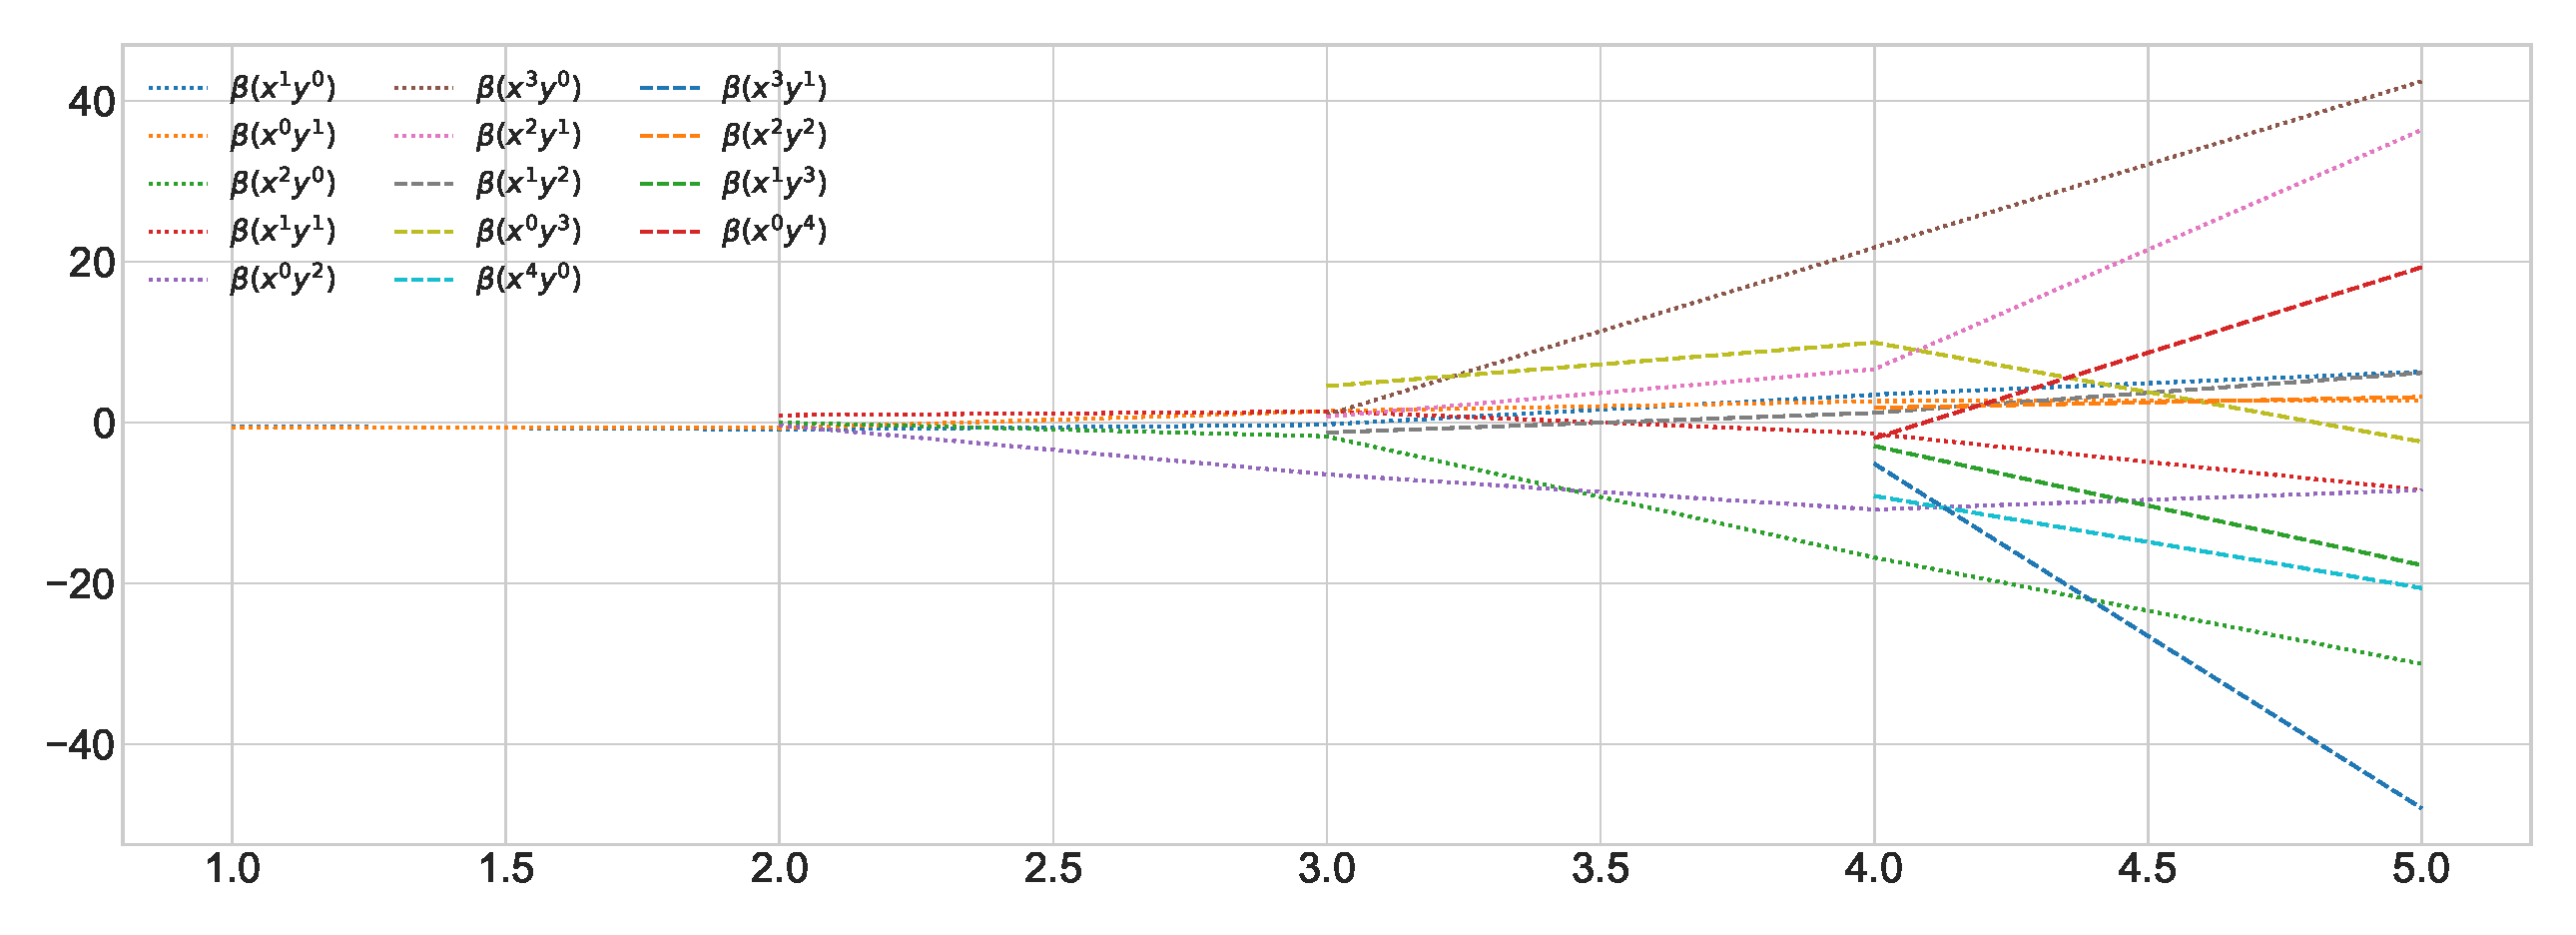
\includegraphics[width=1\linewidth]{images/part_a_beta_vals.pdf}
    \caption{The values for $\boldsymbol{\beta}$ fitted to a data set generated from the Franke function, plotted against polynomial order.}
    \label{fig:part_a_beta_vals}
\end{figure}

\begin{figure}
    \centering
    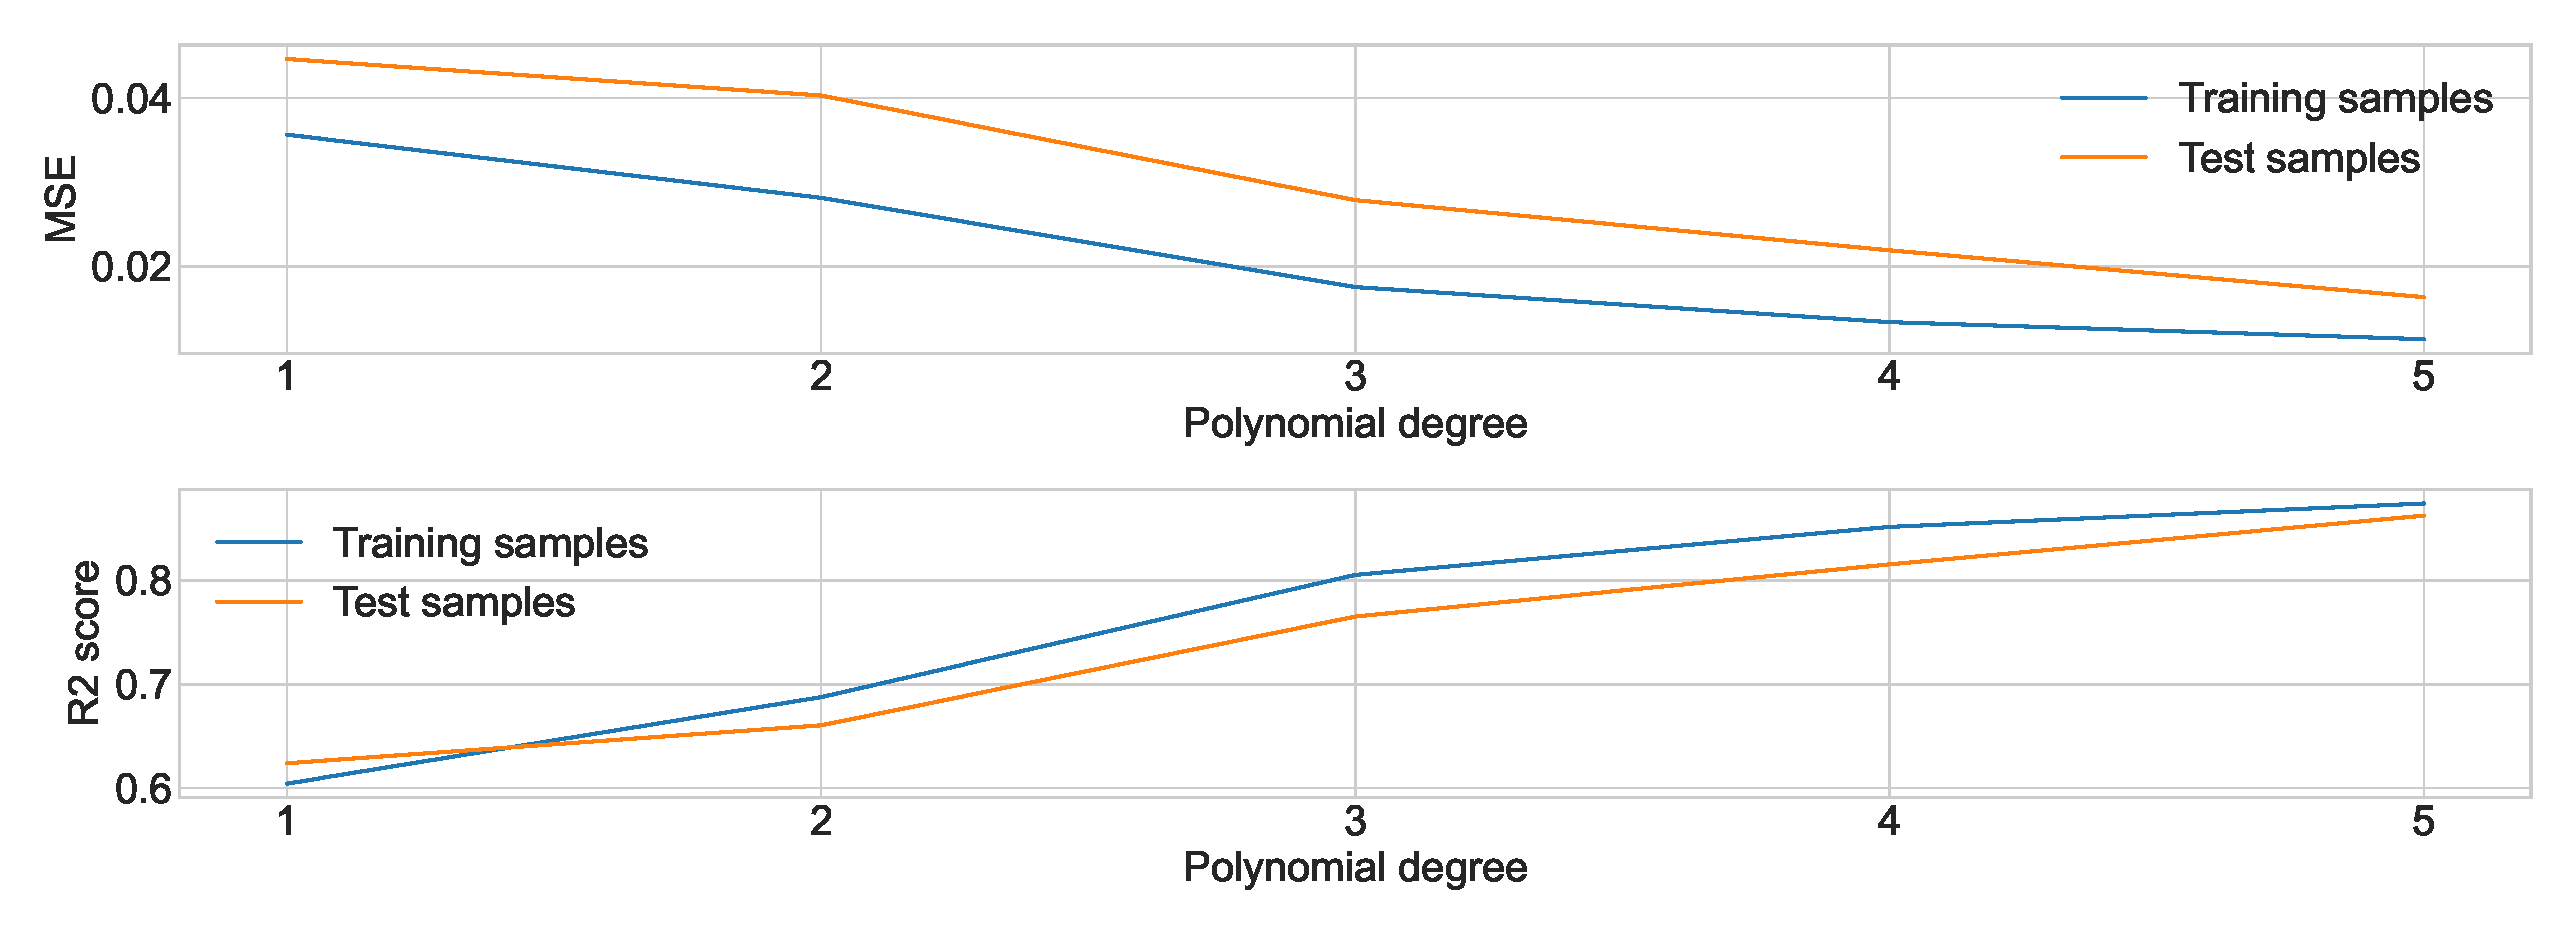
\includegraphics[width=1\linewidth]{images/part_a_MSE_and_r2score_deg5.pdf}
    \caption{The mean squared error and $R^2$-score for OLS predictions on the training and test samples, plotted against polynomial degree of the assumed function.}
    \label{fig:part_a_MSE_and_r2score_deg5}
\end{figure}

Taking one step further, the same results for the $\boldsymbol{\beta}$ values as above are shown in \autoref{fig:part_b_beta_vals}, but now using Ridge regression. We see that the magnitude of the the $\boldsymbol{\beta}$ values for Ridge regression is compressed, compared to the $\boldsymbol{\beta}$ values for OLS. The corresponding plots for MSE and $R^2$ score are shown in \autoref{fig:part_b_MSE_deg5} and \autoref{fig:part_b_r2score_deg5}, respectively. We still see a decrease in error and increase in $R^2$ score for the higher order polynomials, although a slightly earlier flattening of the curves for higher values of $\lambda$ for the test samples. 

\begin{figure}
    \centering
    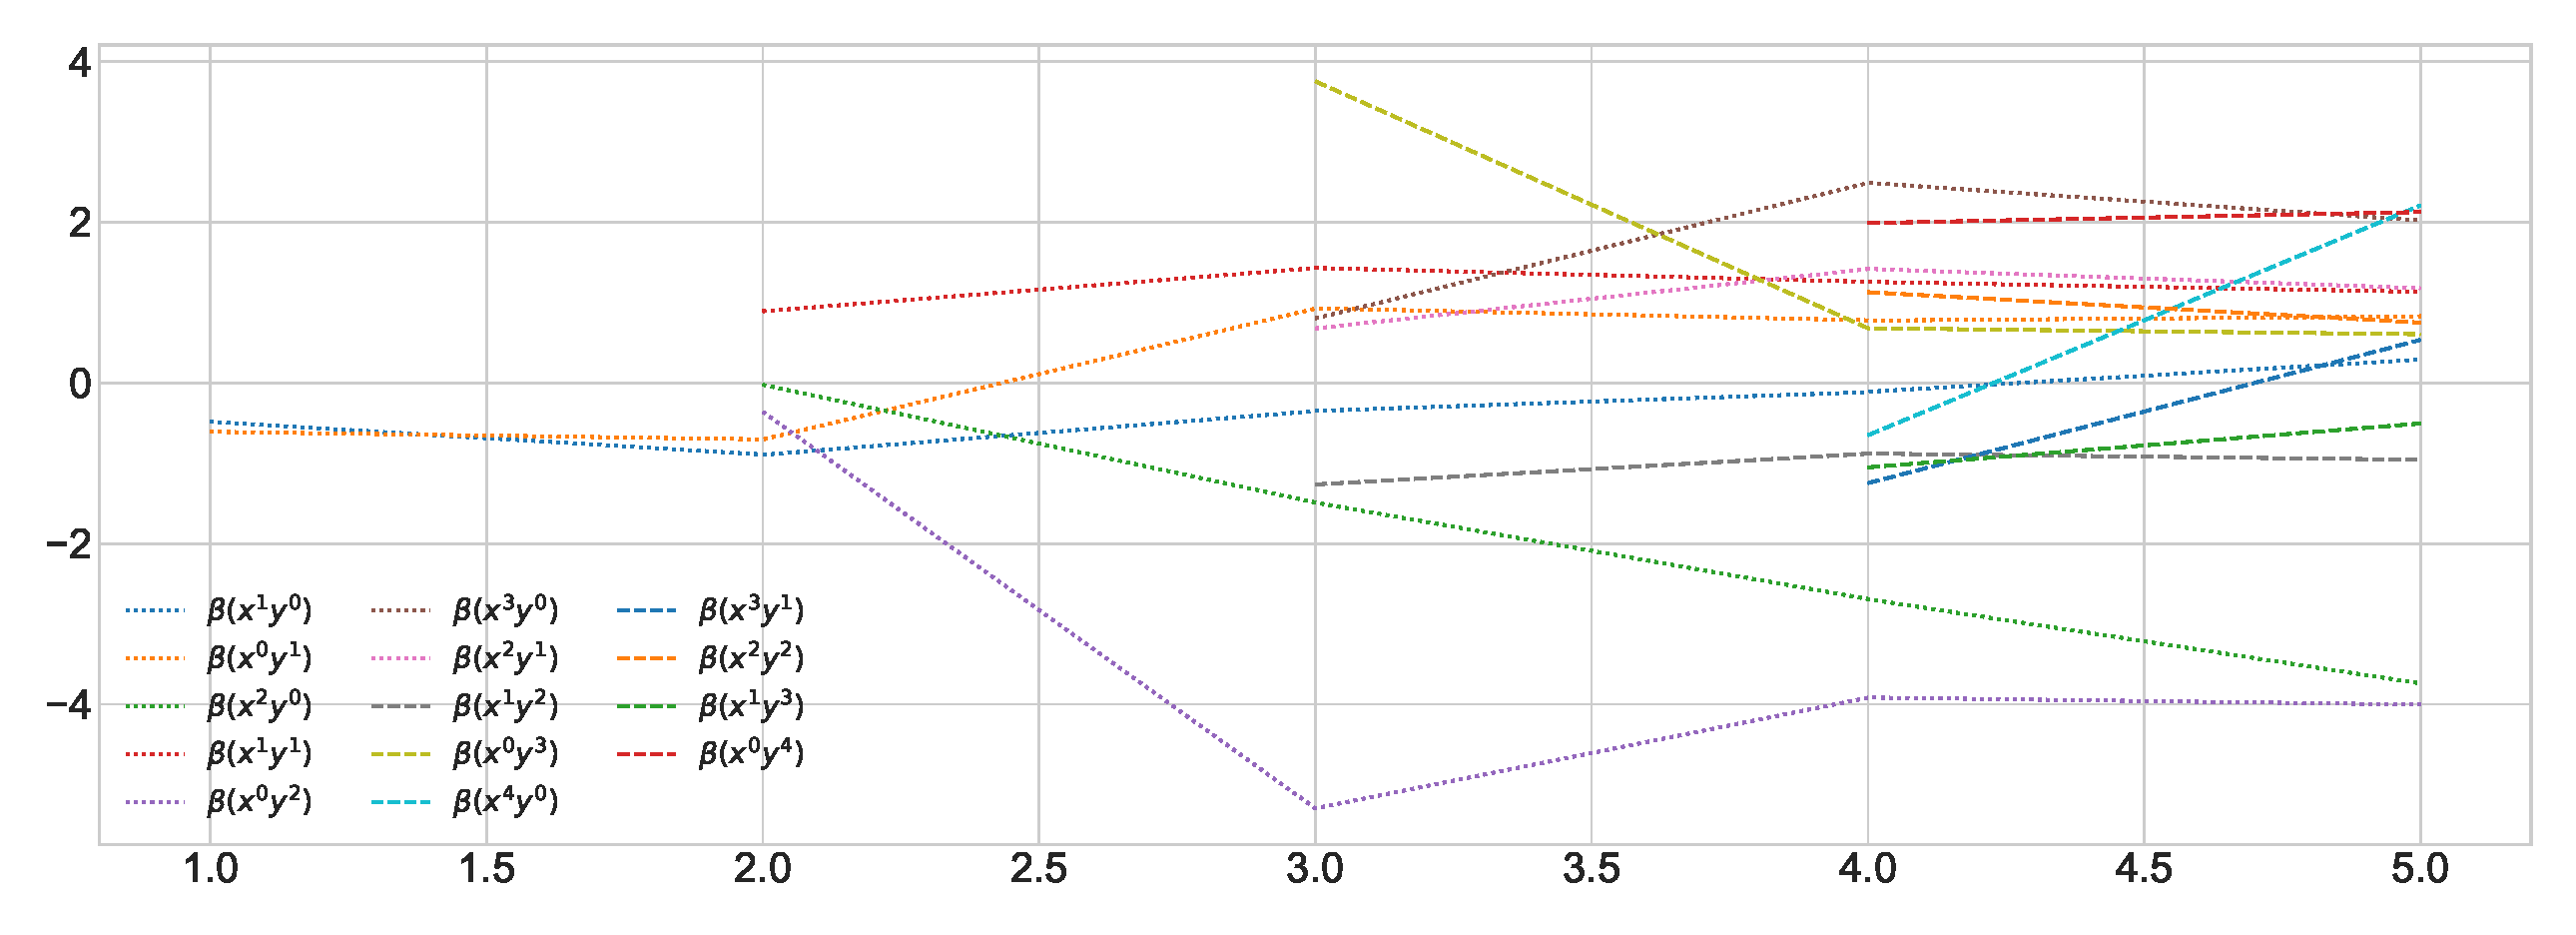
\includegraphics[width=1\linewidth]{images/part_b_beta_vals.pdf}
    \caption{The same $\boldsymbol{\beta}$ values as in \autoref{fig:part_a_beta_vals}} only now with Ridge regression instead of OLS.
    \label{fig:part_b_beta_vals}
\end{figure}

\begin{figure}
    \centering
    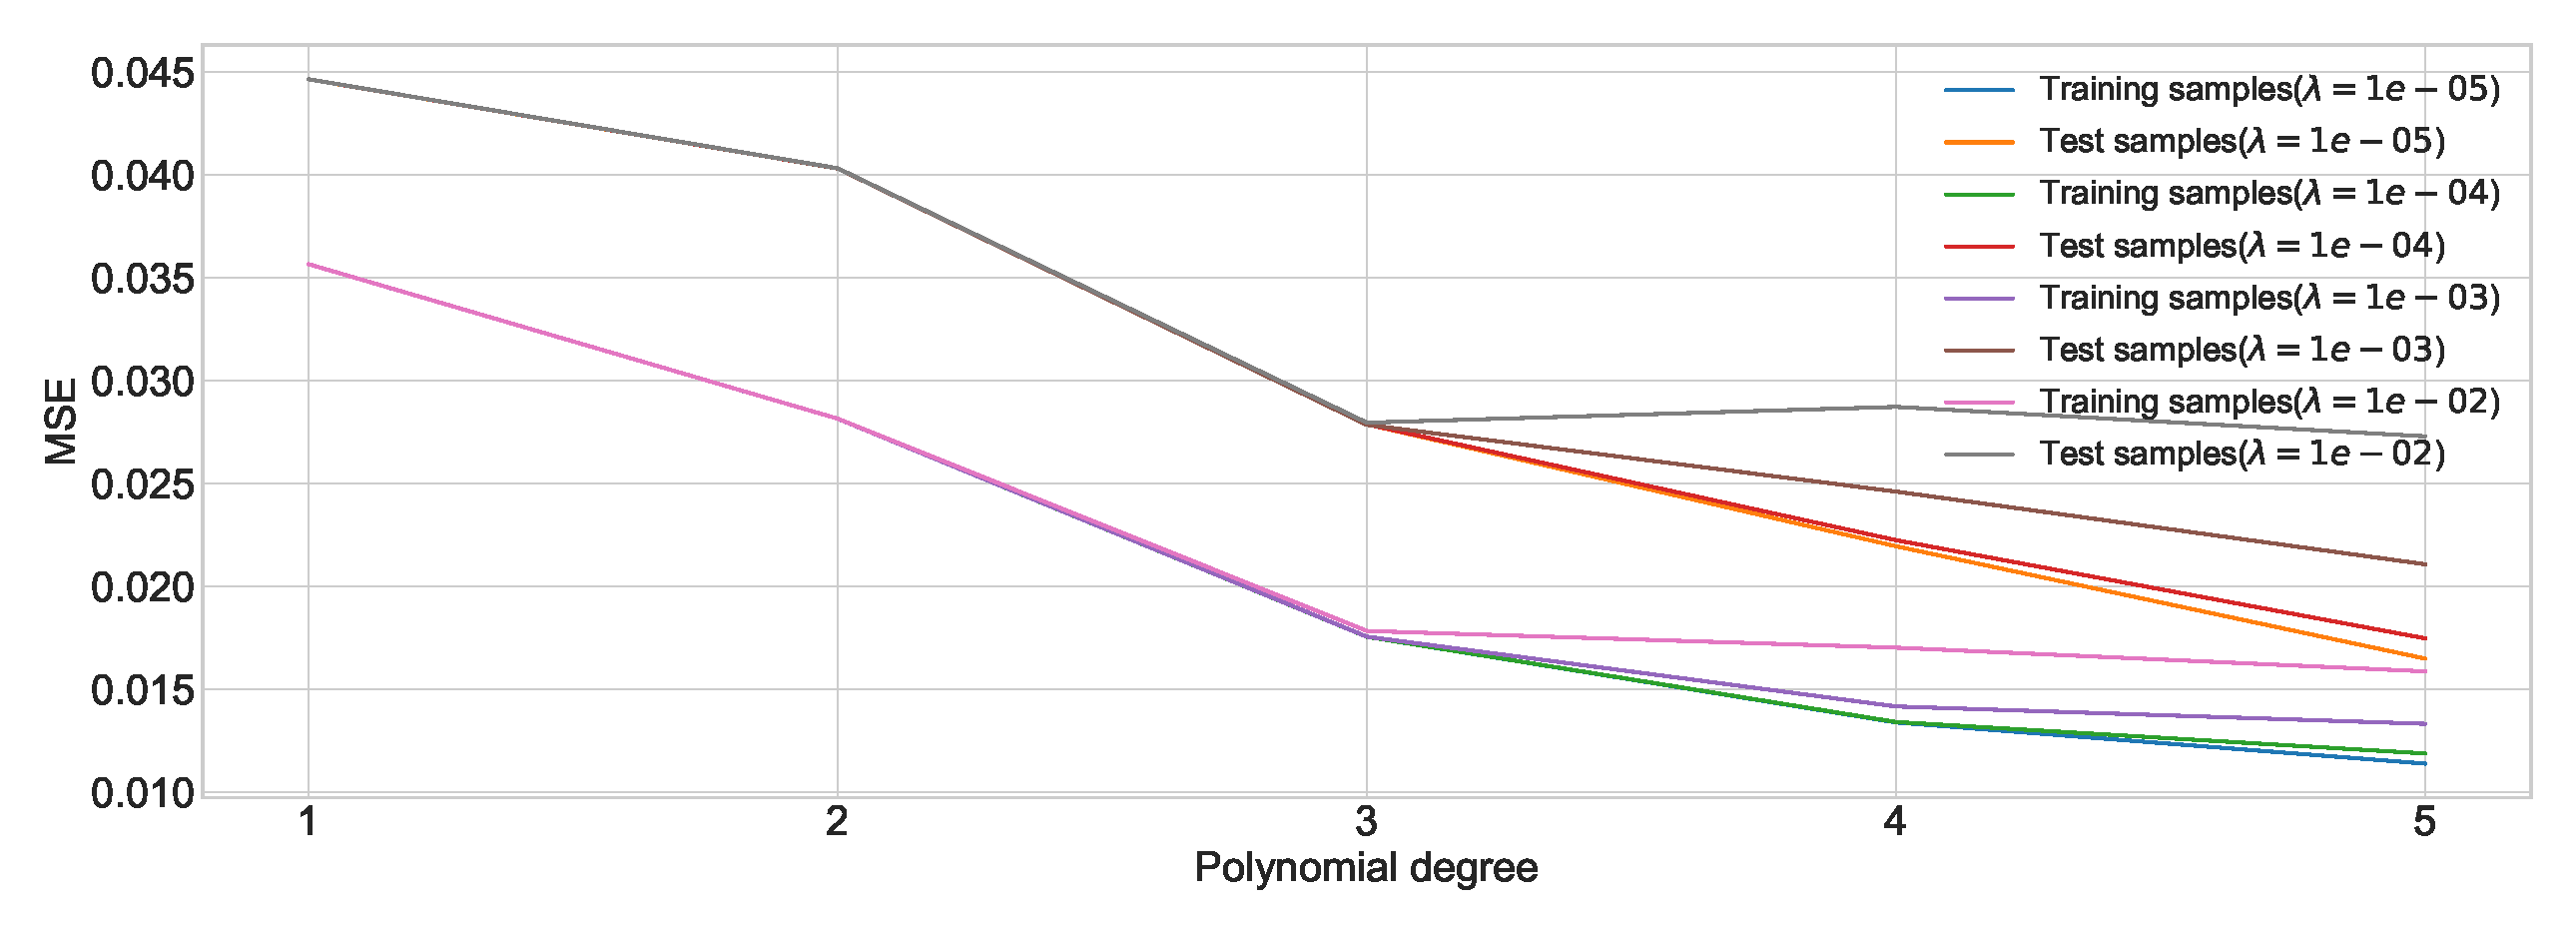
\includegraphics[width=1\linewidth]{images/part_b_MSE_deg5.pdf}
    \caption{The MSE plotted against polynomial degree, for different values of $\lambda$. The underlying function is a fit to the Franke function, using Ridge regression.}
    \label{fig:part_b_MSE_deg5}
\end{figure}

\begin{figure}
    \centering
    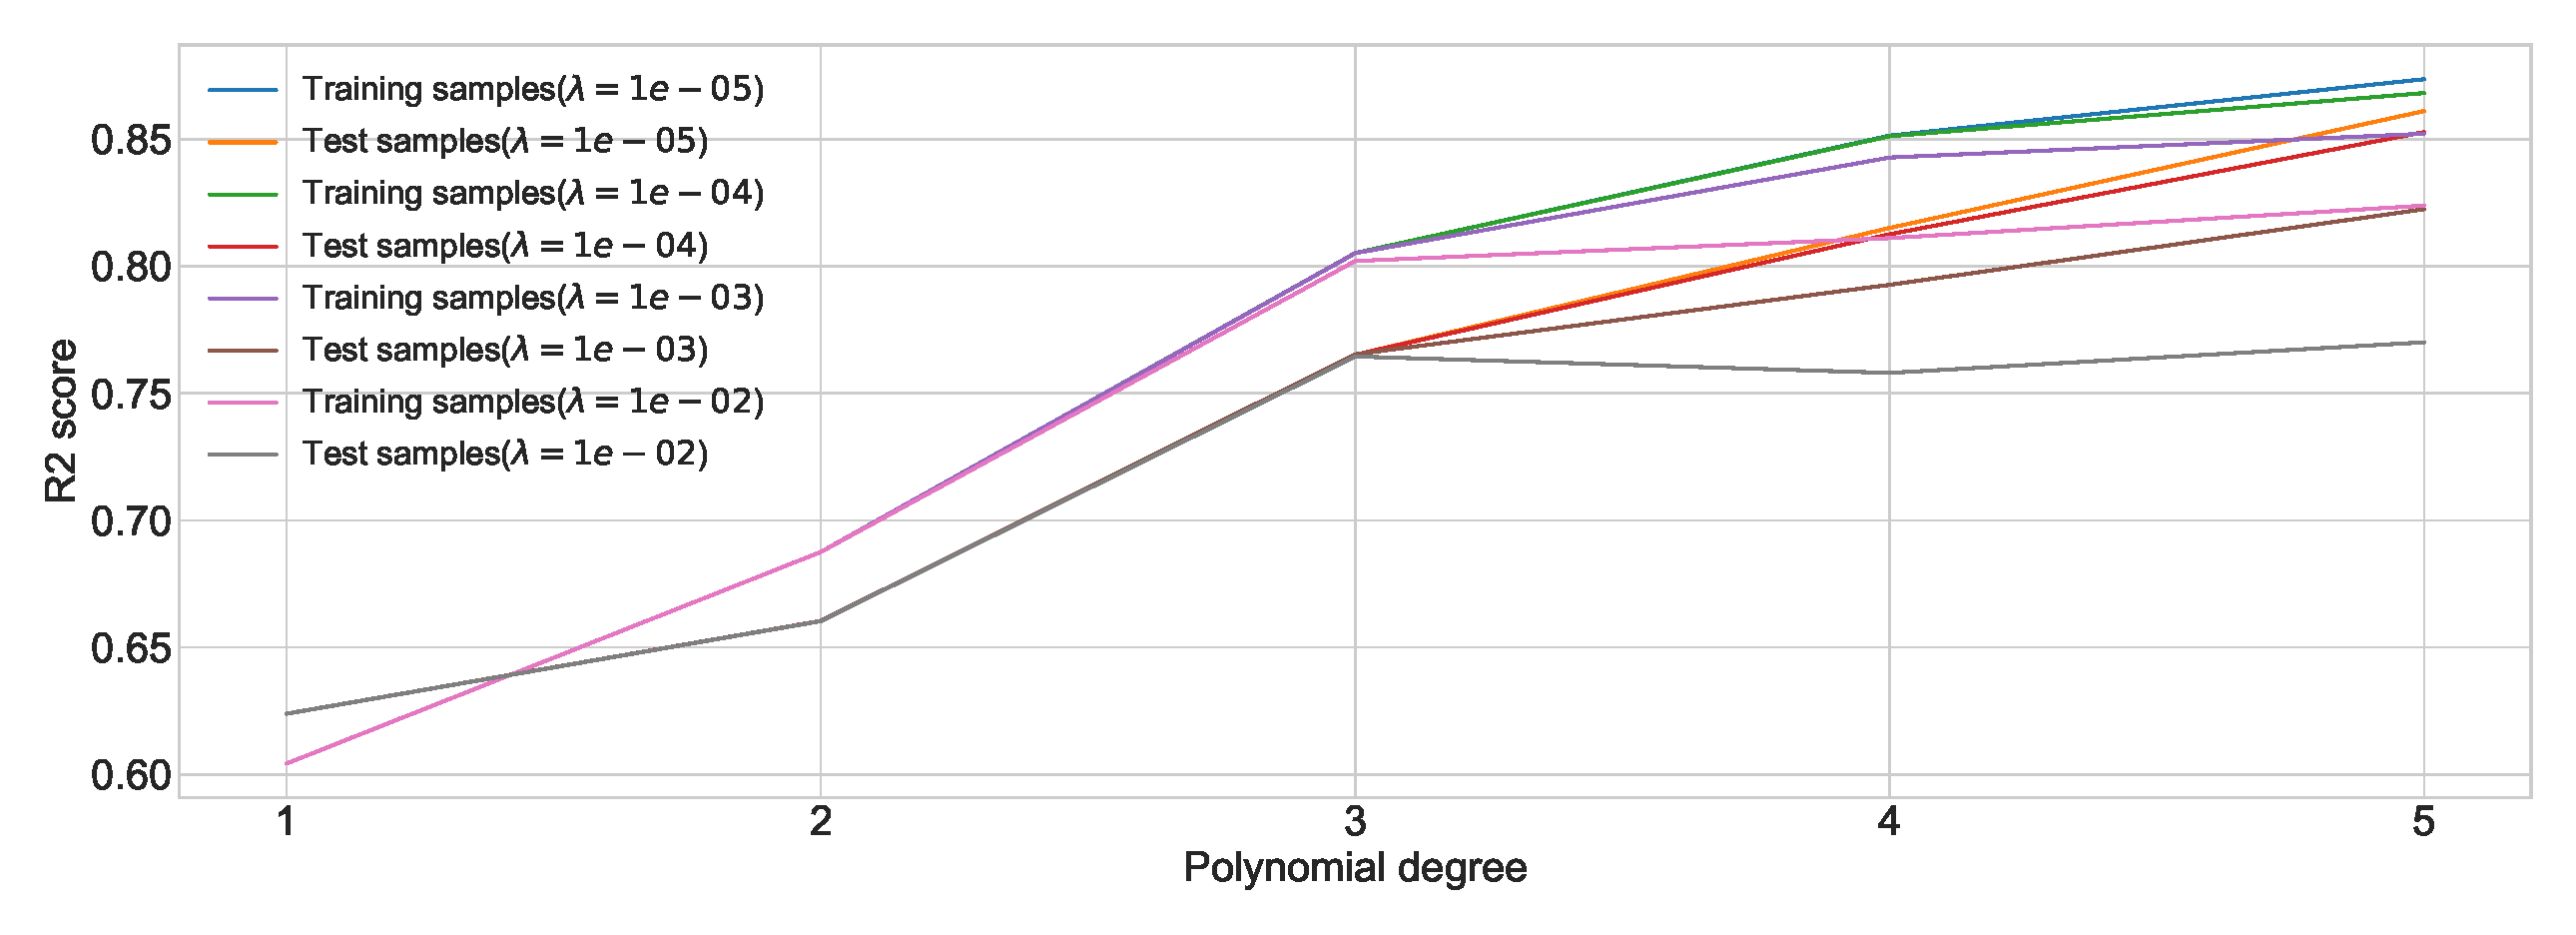
\includegraphics[width=1\linewidth]{images/part_b_r2score_deg5.pdf}
    \caption{The $R^2$ score, plotted against polynomial degree, for different values of $\lambda$. The underlying function is a fit to the Franke function, using Ridge regression.}
    \label{fig:part_b_r2score_deg5}
\end{figure}

We also fit the samples using Lasso regression, where the MSE and $R^2$ results are shown in \autoref{fig:part_c_MSE_deg5} and \autoref{fig:part_c_r2score_deg5}. The figures still show the general trend of a decrease in error and increase in R2 score with increasing complexity of the model, with lower values of $\lambda$ performing the best. However, the steepest increase in performance comes from increasing the polynomial degree to three, with the decrease in error tapering off more slowly for higher order polynomials.  

\begin{figure}
    \centering
    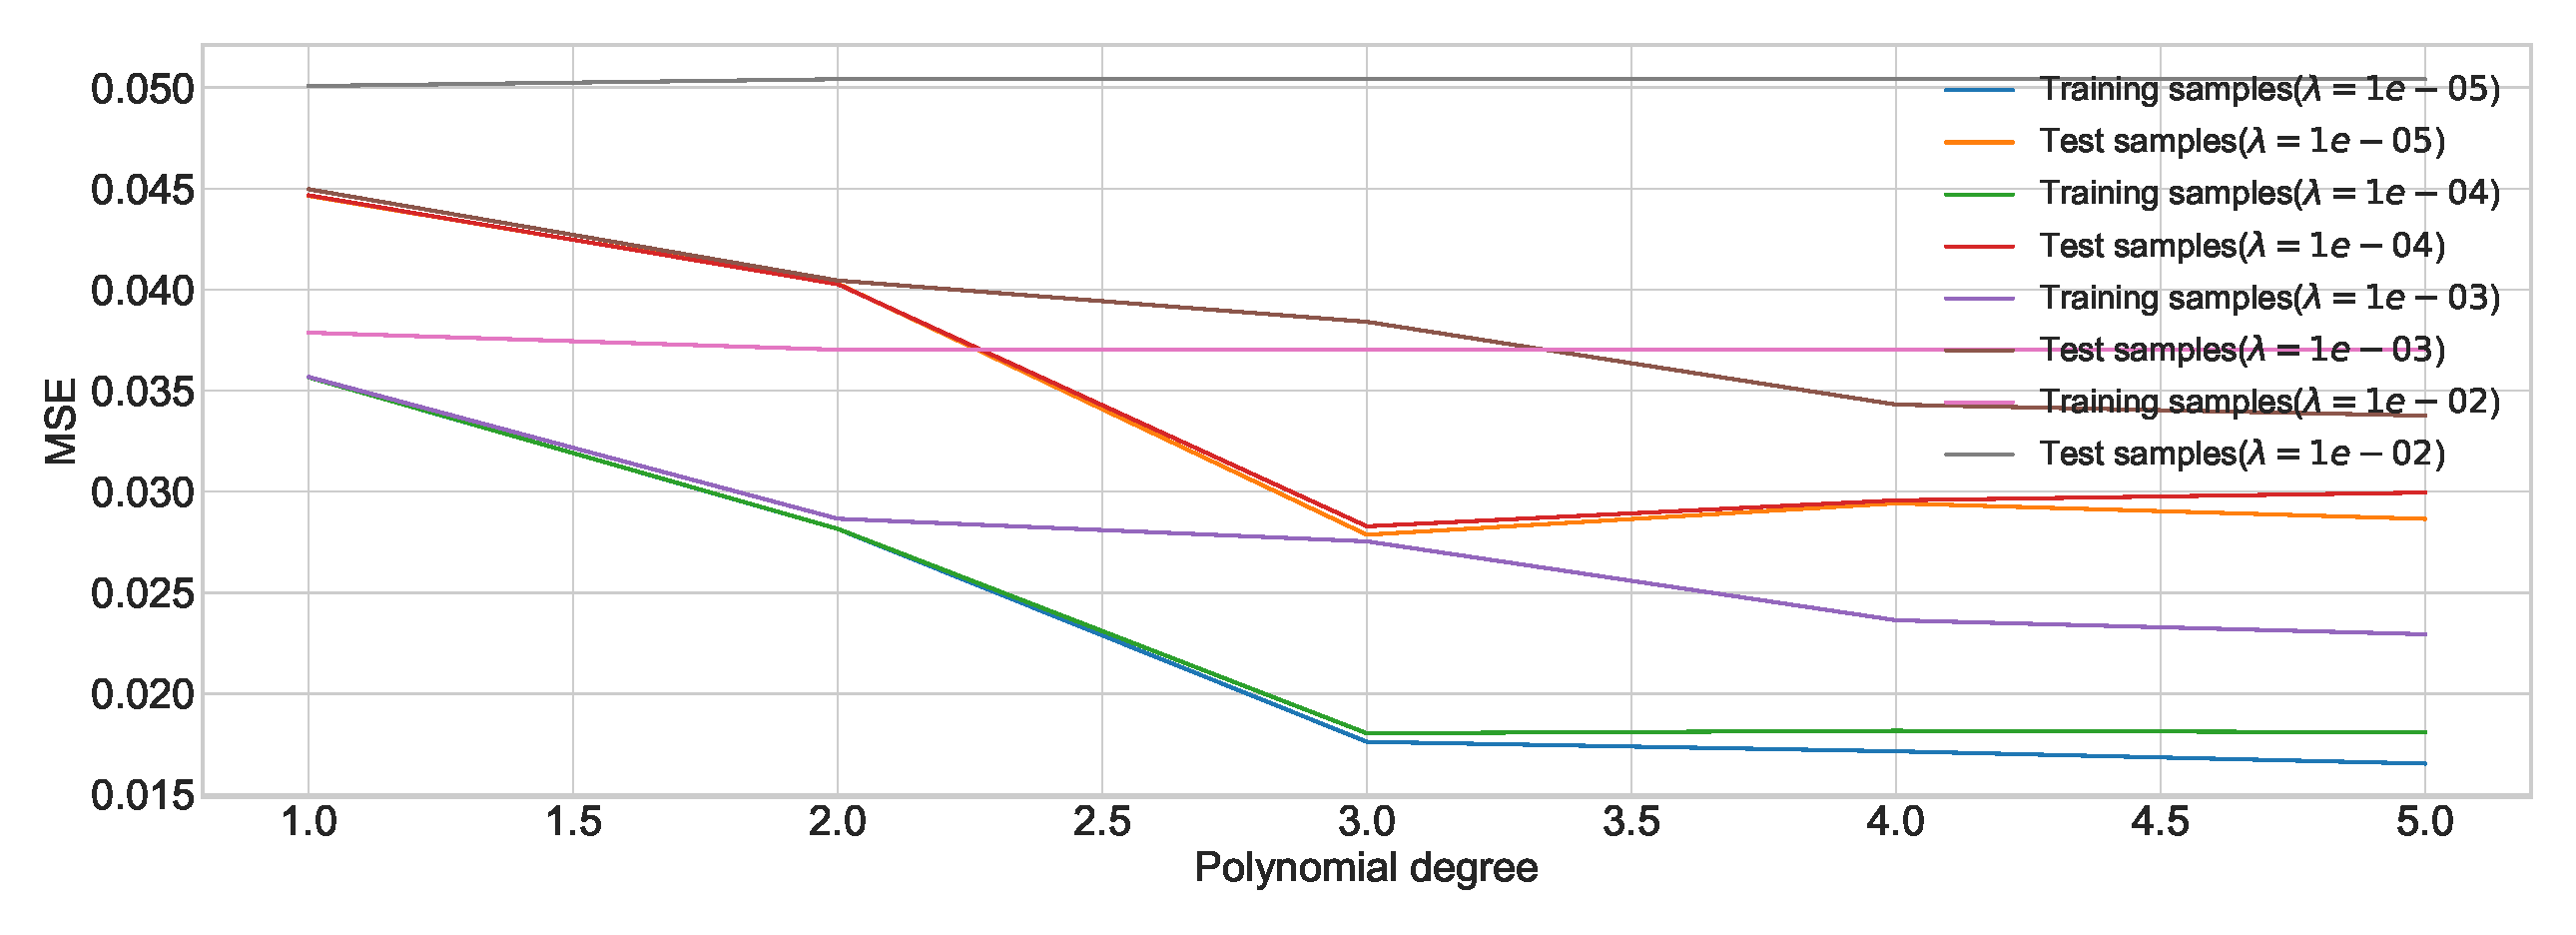
\includegraphics[width=1\linewidth]{images/part_c_MSE_deg5.pdf}
    \caption{The MSE plotted against polynomial degree, for different values of $\lambda$. The underlying function is a fit to the Franke function, using Lasso regression.}
    \label{fig:part_c_MSE_deg5}
\end{figure}

\begin{figure}
    \centering
    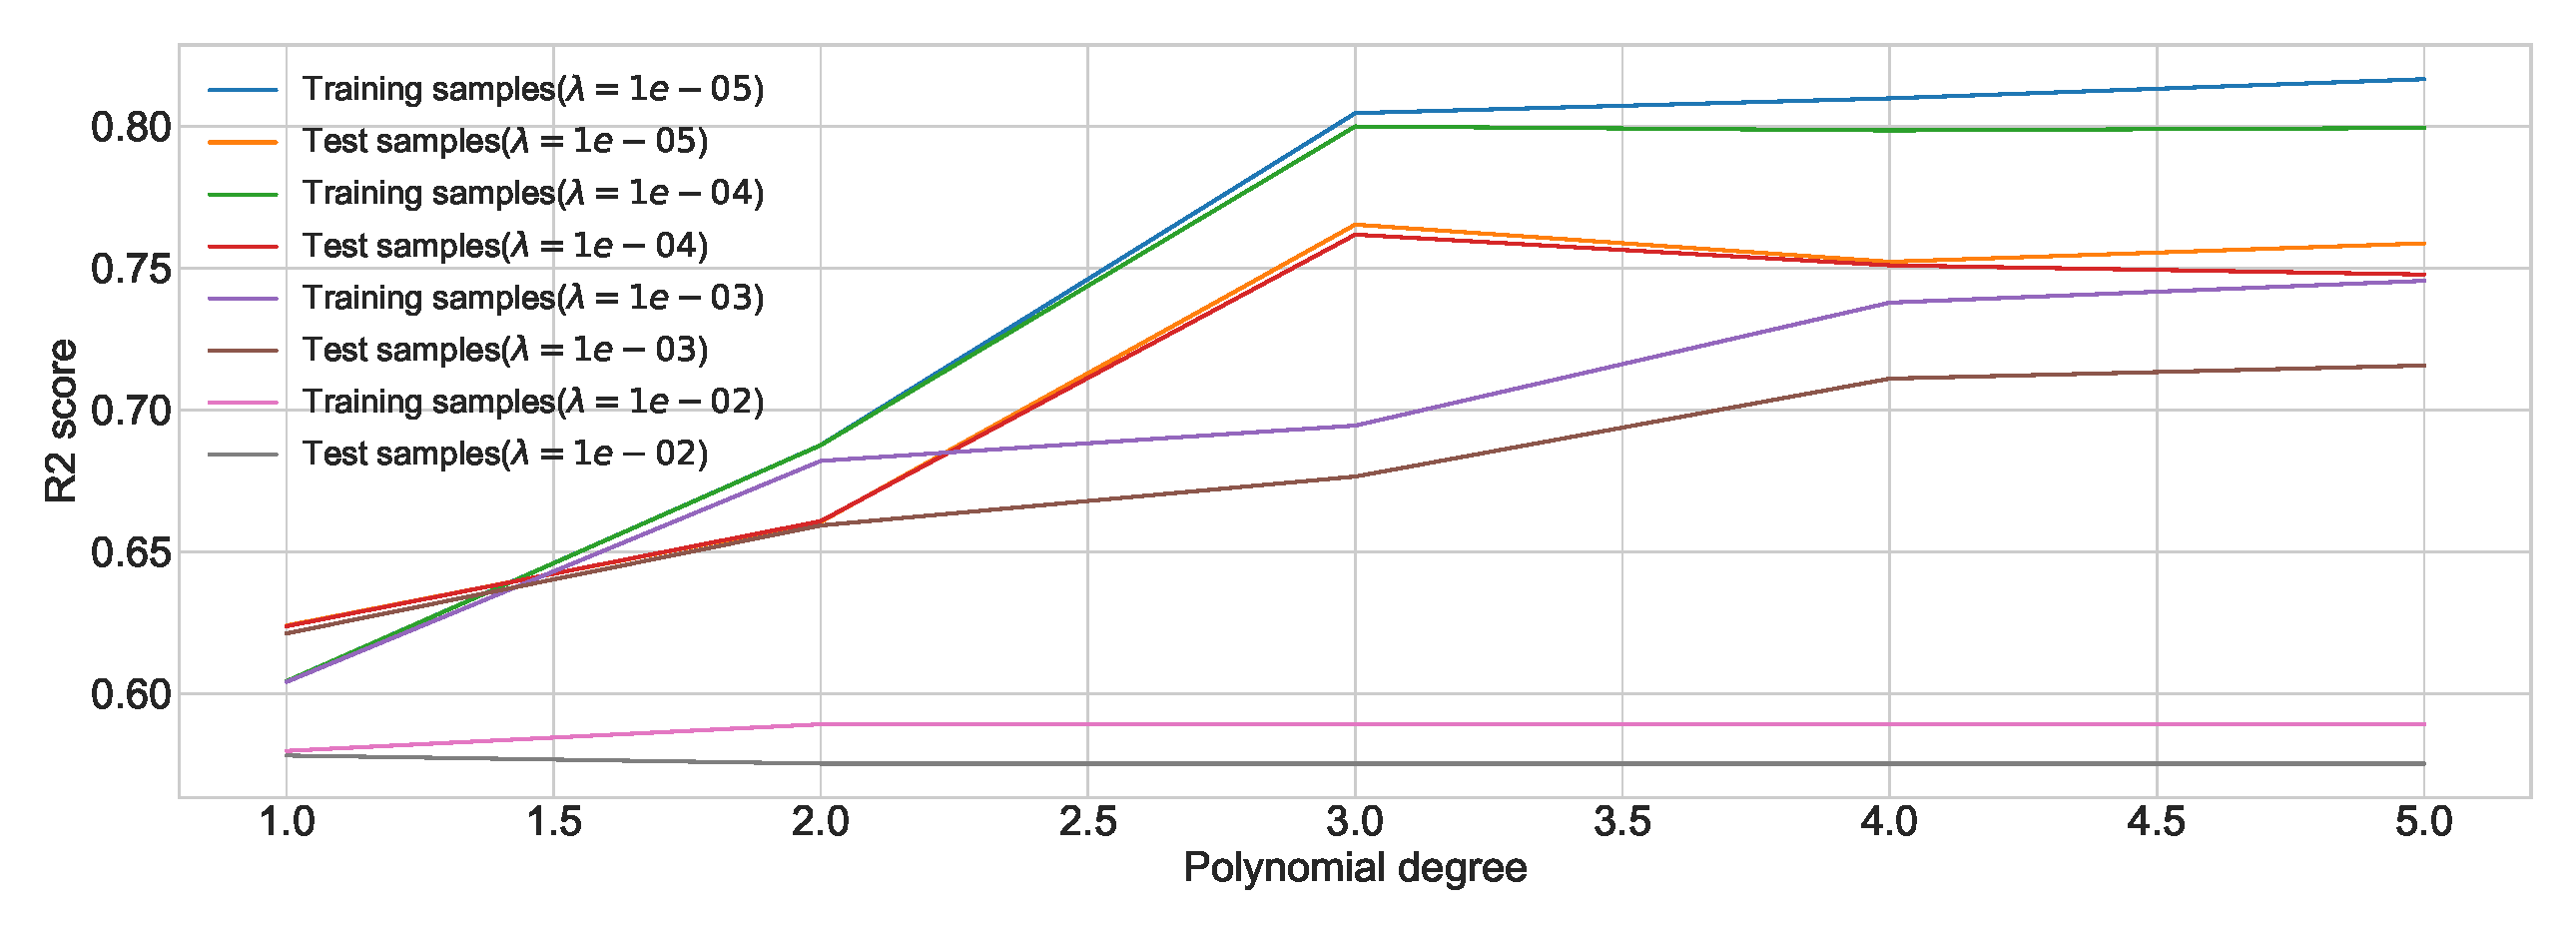
\includegraphics[width=1\linewidth]{images/part_c_r2score_deg5.pdf}
    \caption{The $R^2$ score plotted against polynomial degree, for different values of $\lambda$. The underlying function is a fit to the Franke function, using Lasso regression.}
    \label{fig:part_c_r2score_deg5}
\end{figure}

In \autoref{fig:part_e_MSE_deg10}, we present the MSE for OLS, plotted as a function of complexity in the form of polynomial order, up to polynomial degree 10. This shows a steady decrease in error for the training samples as expected. The error for the test data is also generally decreasing as a function of complexity, but might exhibit a small upwards trend for the highest order polynomials. 

\begin{figure}
    \centering
    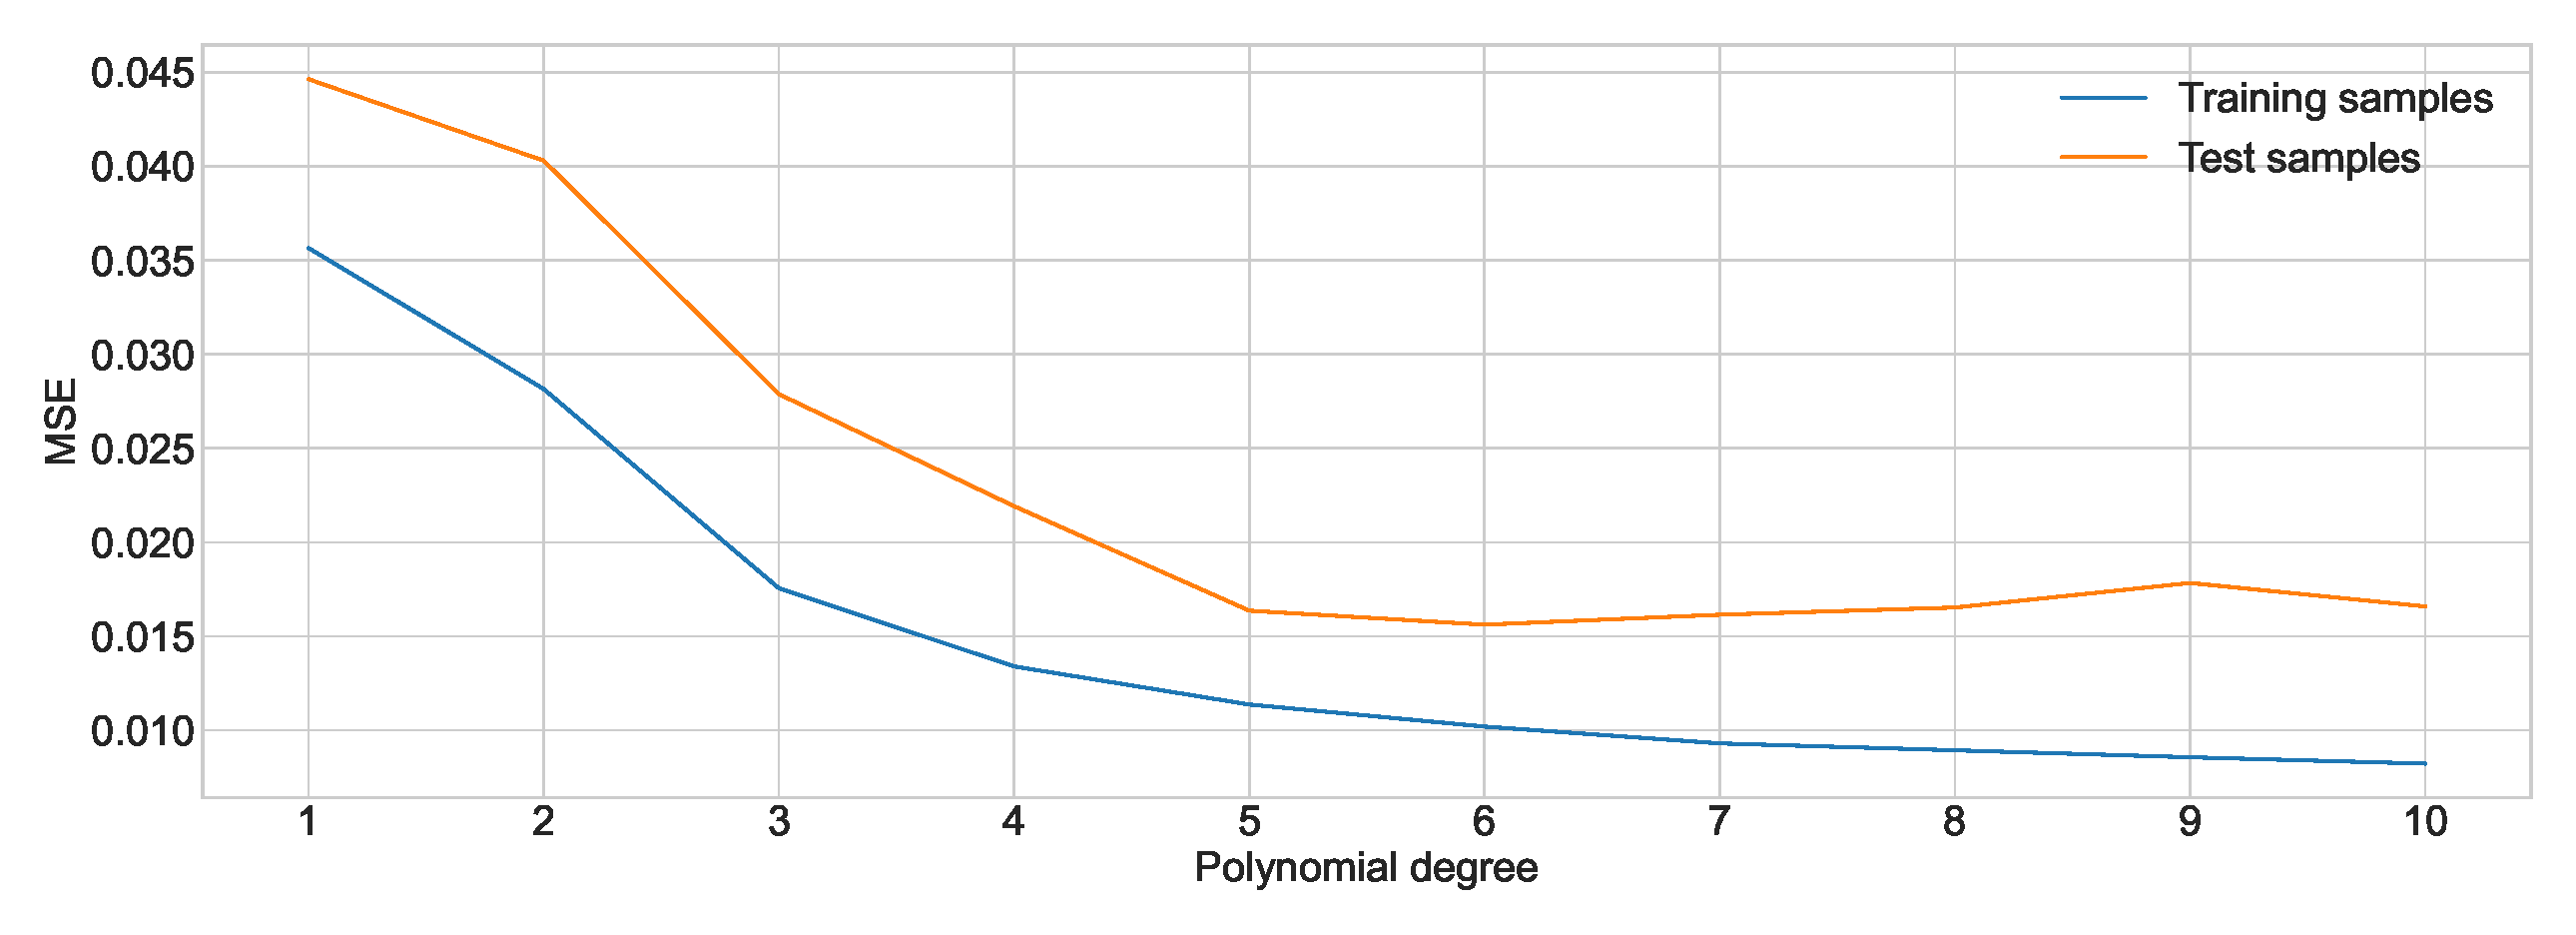
\includegraphics[width=1\linewidth]{images/part_e_MSE_deg10.pdf}
    \caption{The mean squared error using OLS for function up to polynomial degree 10. The MSE for the training data continues to shrink as a function of complexity, while the MSE for test data reaches a plateau and begins slightly increasing.}
    \label{fig:part_e_MSE_deg10}
\end{figure}

In \autoref{fig:part_e_bias_var_21x21} and \autoref{fig:part_e_bias_var_101x101}, we show the MSE as a function of complexity, along with the plot of its constituent parts, the bias and variance. The bootstrap resampling method has been applied for both results. \autoref{fig:part_e_bias_var_21x21} originated from the data set of size $21 \times 21$, while the data set of size $101 \times 101$ was used in \autoref{fig:part_e_bias_var_101x101}. For the smaller data set, we can see a clear indication of the variance increasing for the higher order polynomials, and a larger part of the total MSE is made up of the variance. For the larger data set, shown in \autoref{fig:part_e_bias_var_101x101}, the total MSE is made up almost exclusively of the bias, and the variance is negligible throughout. 

\begin{figure}
    \centering
    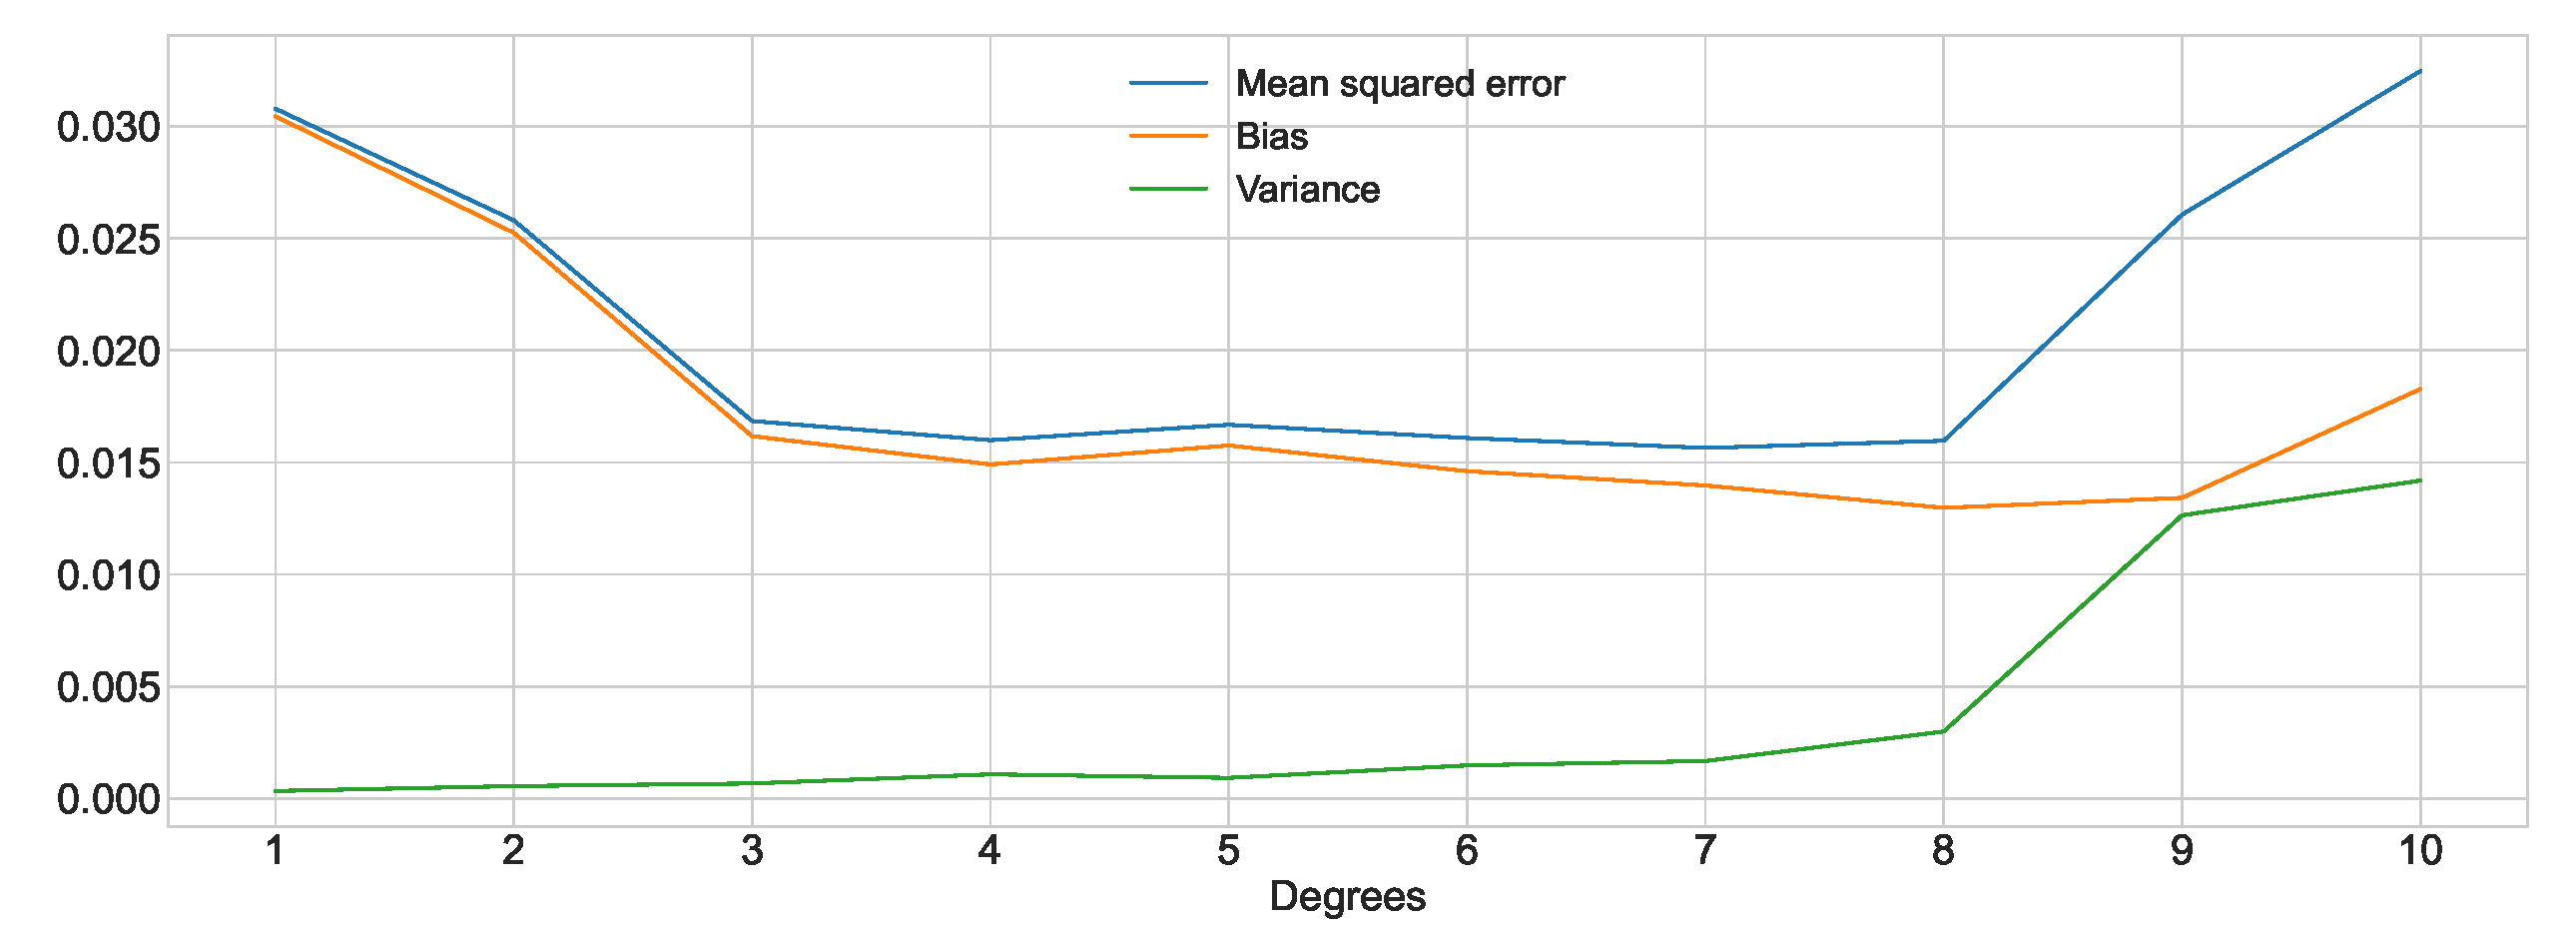
\includegraphics[width=1\linewidth]{images/part_e_bias_var_21x21.pdf}
    \caption{The bias and variance terms in \autoref{eq:bias-variance}, as well as the total mean squared error plotted as function of polynomial degree. These values were calculated by performing bootstrap resampling 10 times with the data set of size $21\times21$.}
    \label{fig:part_e_bias_var_21x21}
\end{figure}

\begin{figure}
    \centering
    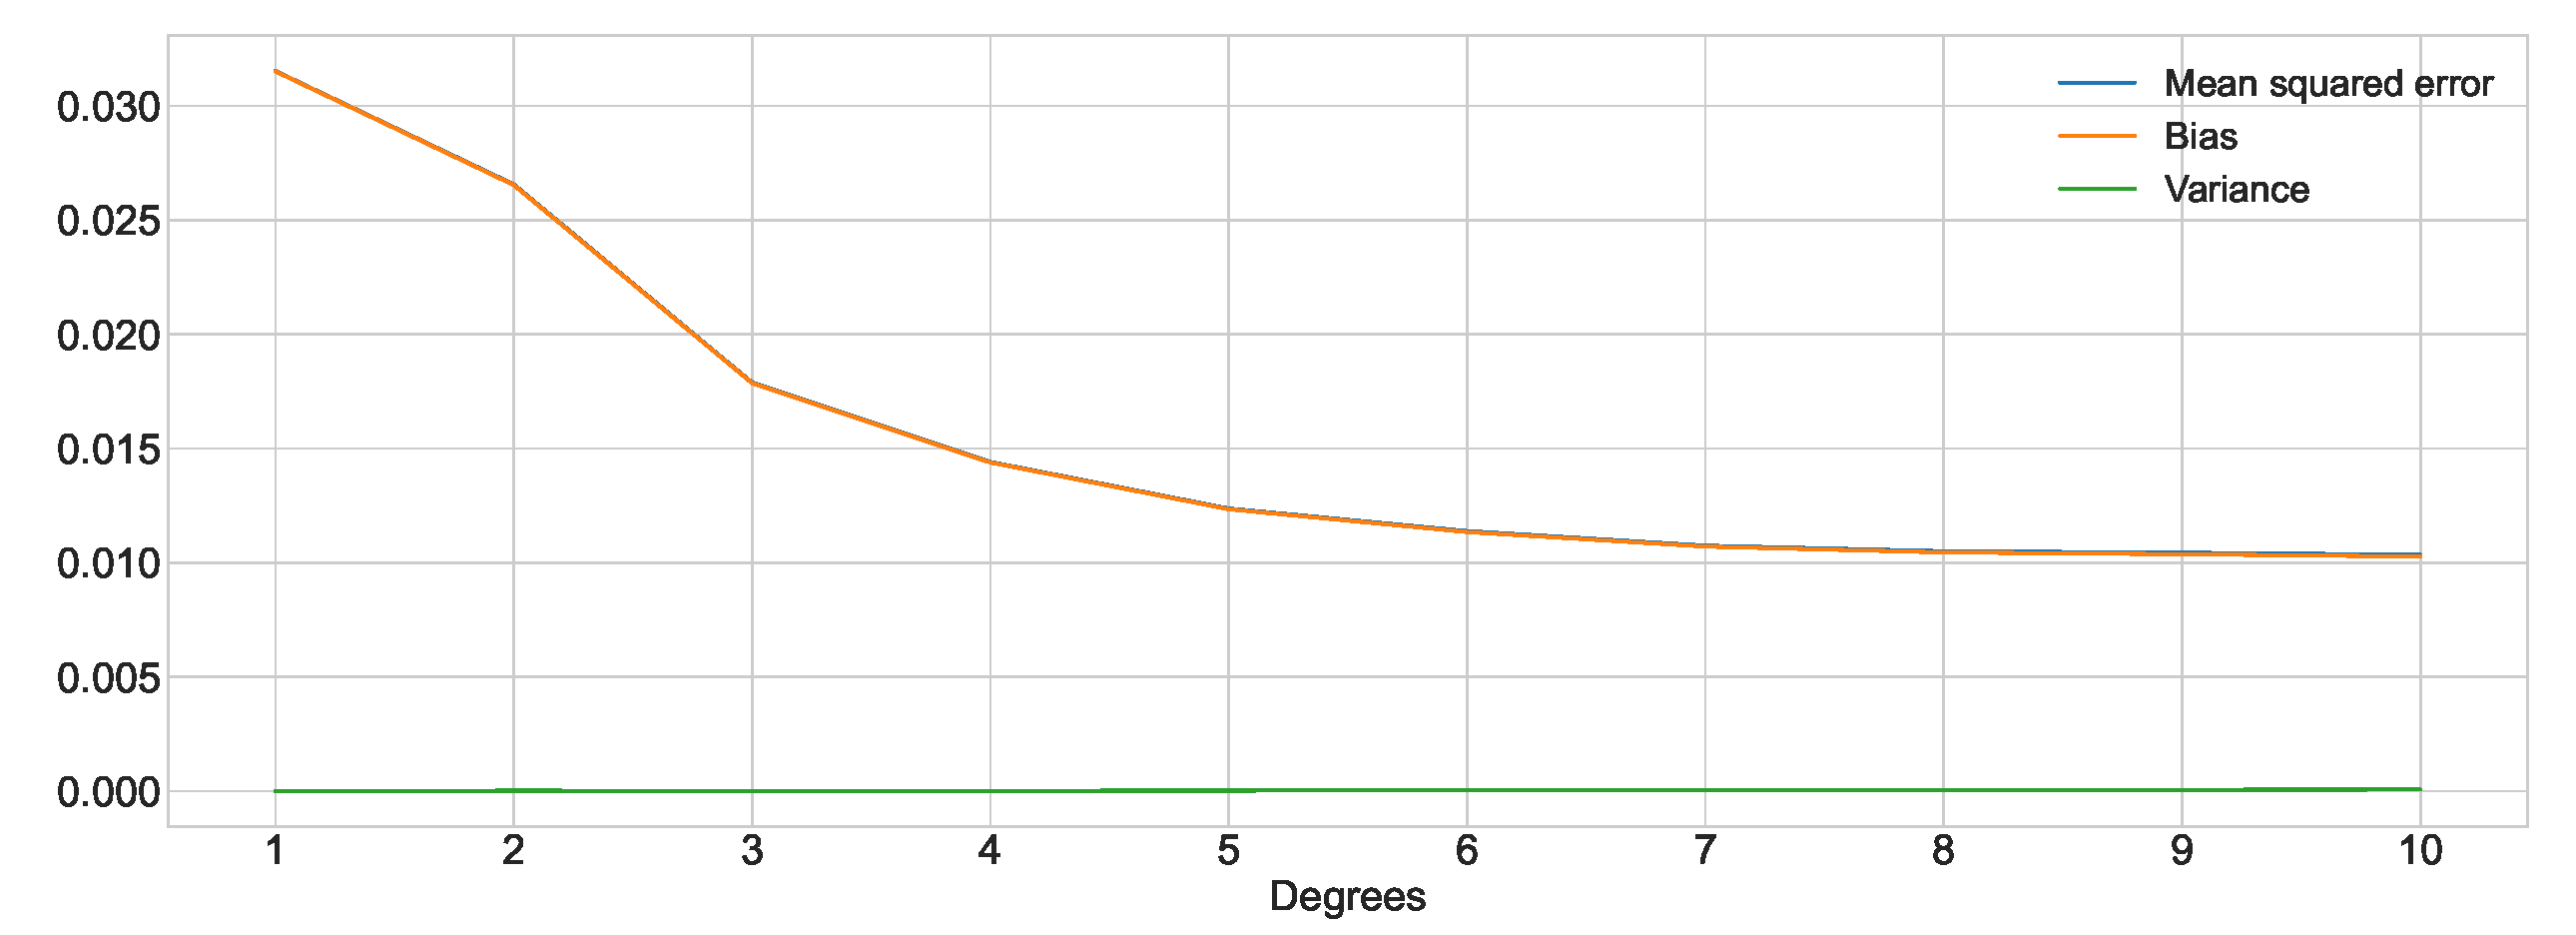
\includegraphics[width=1\linewidth]{images/part_e_bias_var_101x101.pdf}
    \caption{The bias and variance terms in \autoref{eq:bias-variance}, as well as the total mean squared error plotted as function of polynomial degree. These values were calculated by performing bootstrap resampling 10 times with the data set of size $101\times101$.}
    \label{fig:part_e_bias_var_101x101}
\end{figure}

We demonstrate a comparison between the bootstrap and cross-validation resampling methods in \autoref{fig:part_f_MSE_10bootstraps_10fold_crossval}. The results show that while the bootstrap method provides lower MSE for lower order polynomials, it is quickly overtaken by cross-validation, as the method yielding the lowest error measure. The bootstrap method shows an increase in error for the highest order polynomials. 

\begin{figure}
    \centering
    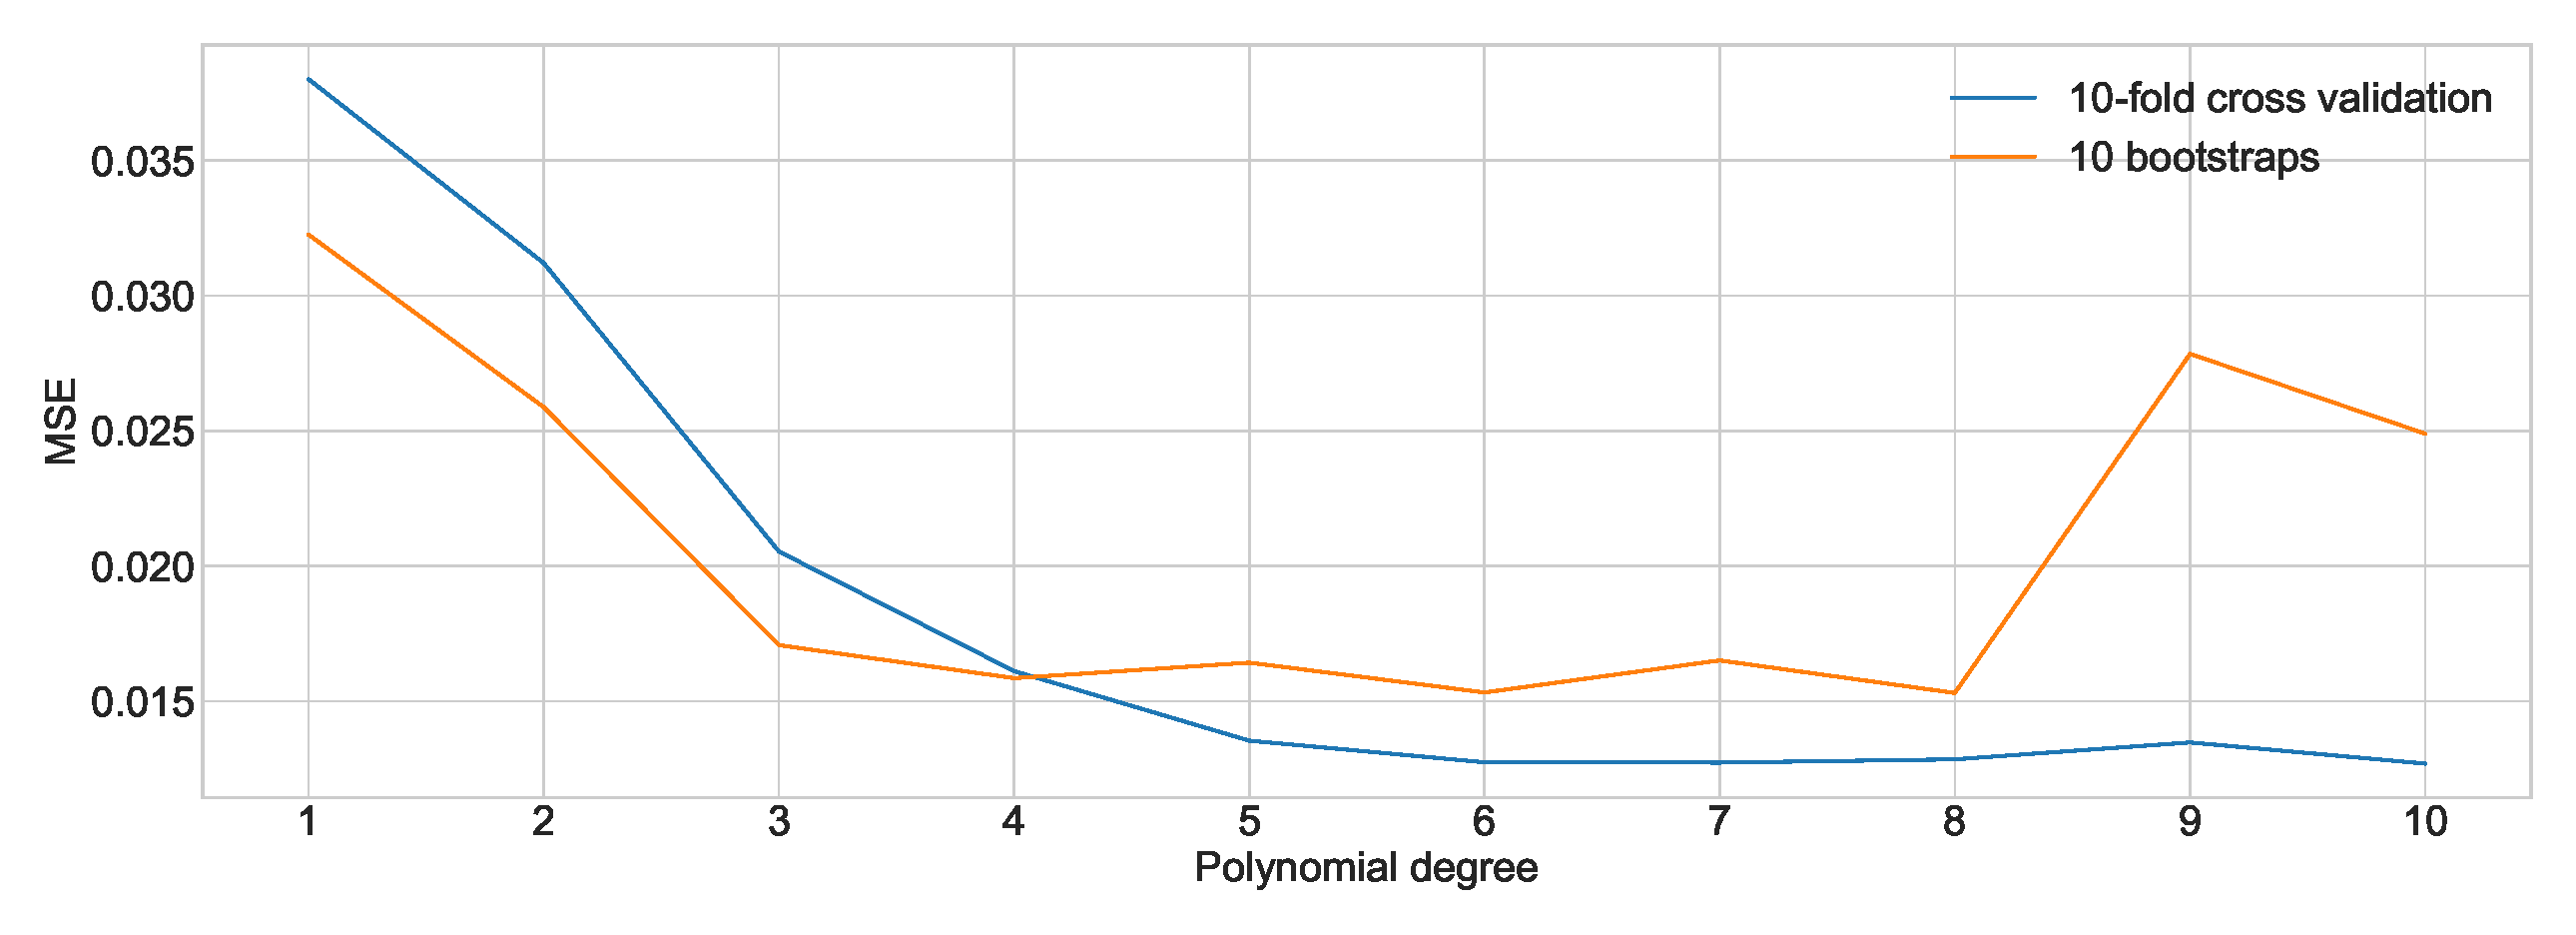
\includegraphics[width=1\linewidth]{images/part_f_MSE_10bootstraps_10fold_crossval.pdf}
    \caption{Comparison between the mean of the MSE from 10 bootstraps and the mean of the MSE from the 10 configurations of the training/test set in 10-fold cross-validation. Both resampling methods were used with ordinary least squares regression.}
    \label{fig:part_f_MSE_10bootstraps_10fold_crossval}
\end{figure}

We present the MSE for different regression methods, using a 10-fold cross-validation, plotted against complexity in \autoref{fig:part_f_MSE_10fold_crossval_ols_ridge_lasso}. Again, OLS provides the lowest MSE, with Ridge regression with small values of $\lambda$ trailing the closest. An interesting observation is that Lasso regression gave the highest MSE, regardless of the value of $\lambda$, when compared to Ridge regression and OLS. 

\begin{figure}
    \centering
    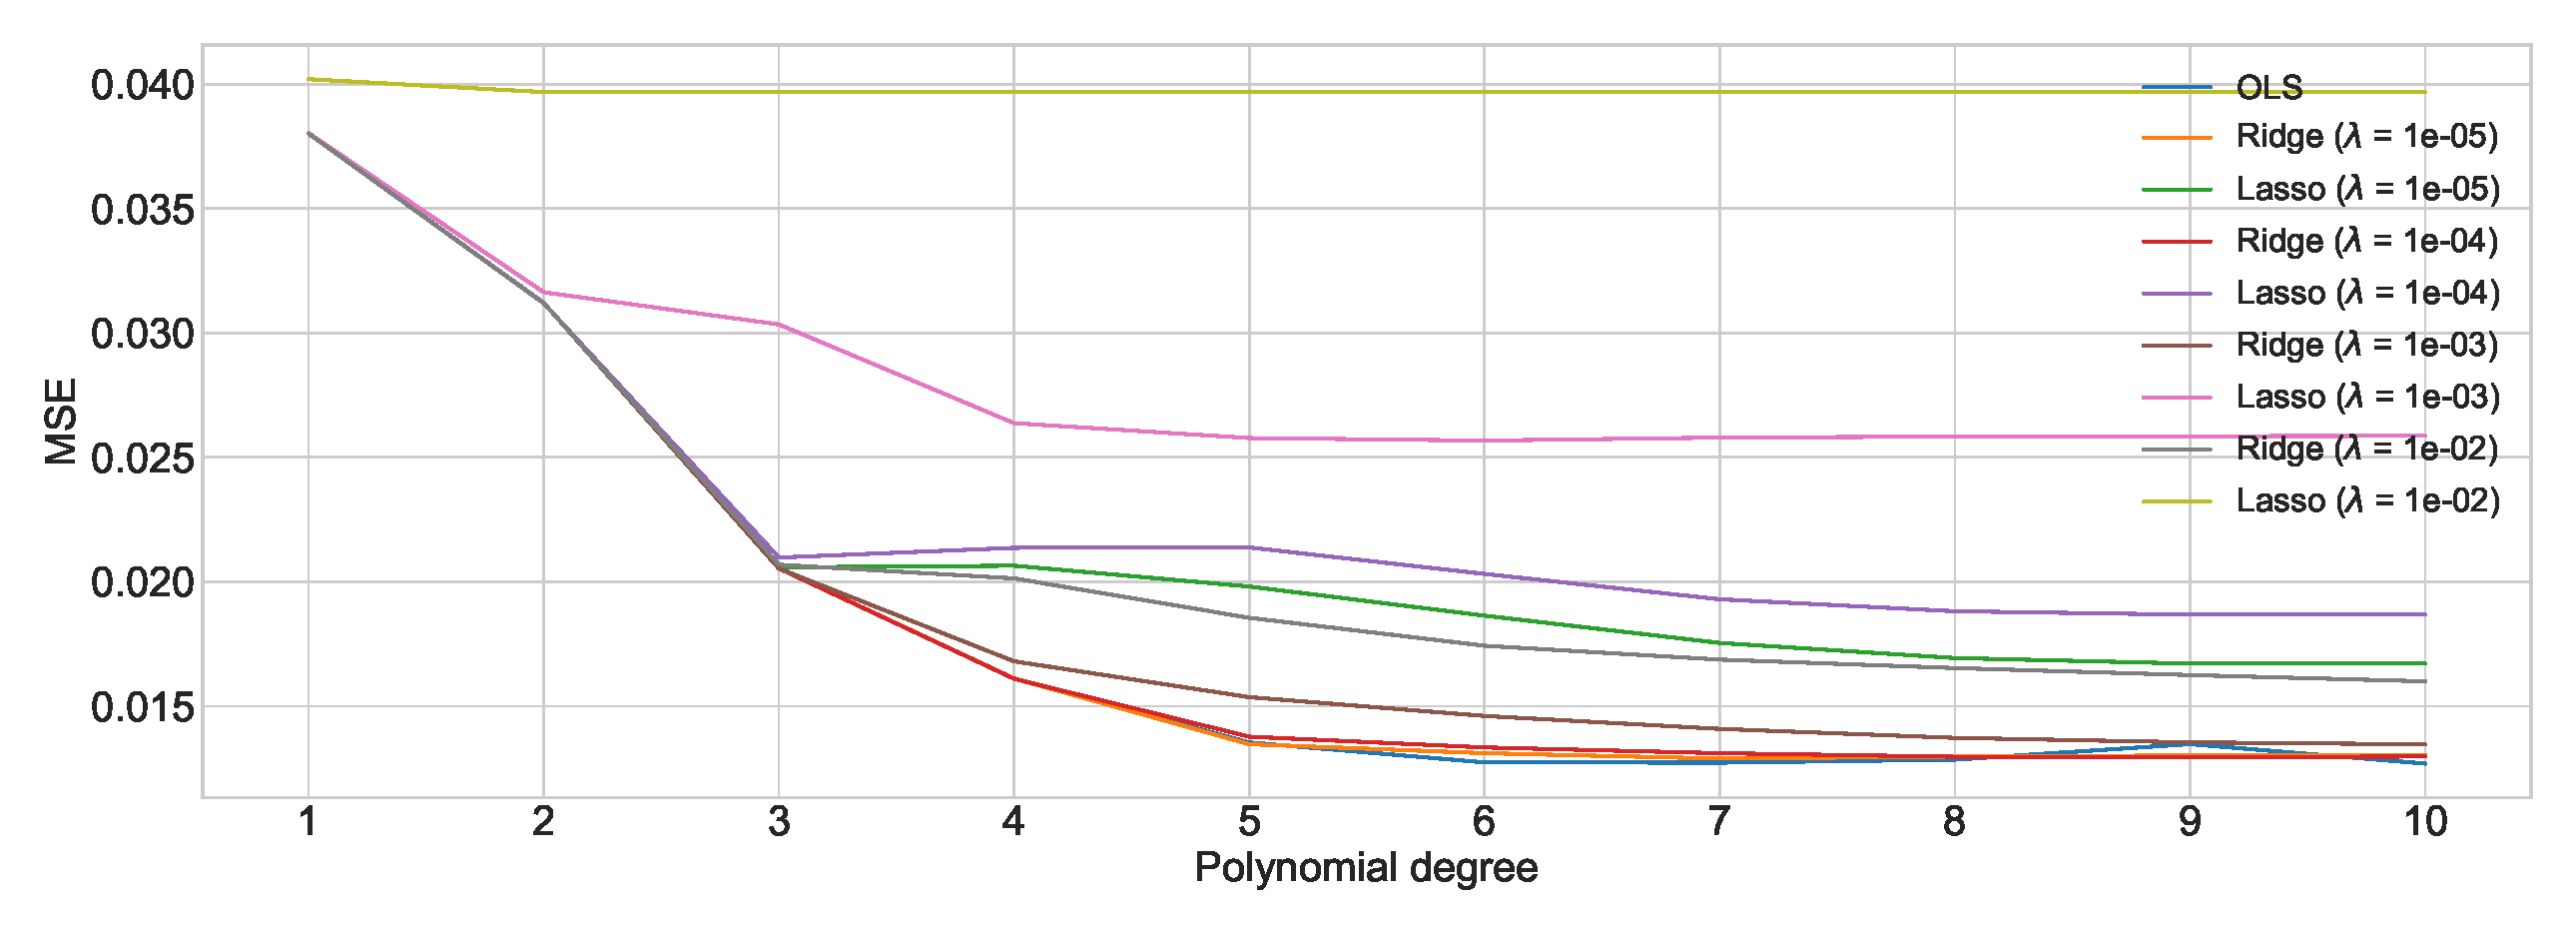
\includegraphics[width=1\linewidth]{images/part_f_MSE_10fold_crossval_ols_ridge_lasso.pdf}
    \caption{The mean of the MSE from 10-fold cross-validation for ordinary least squares, Ridge and Lasso regression, plotted against the polynomial degree.}
    \label{fig:part_f_MSE_10fold_crossval_ols_ridge_lasso}
\end{figure}

Finally, we show the application of the regression models to real-world data in \autoref{fig:part_g_real_data_mse_ols_ridge_lasso}. Note that the scale for the MSE is different, as we only centered our data, but did not normalize them. Again, the results show that OLS consistently gave the lowest MSE, followed by Ridge regression. Also, pay attention to the three results for Lasso regression, which all lie roughly along the same line. 

\begin{figure}
    \centering
    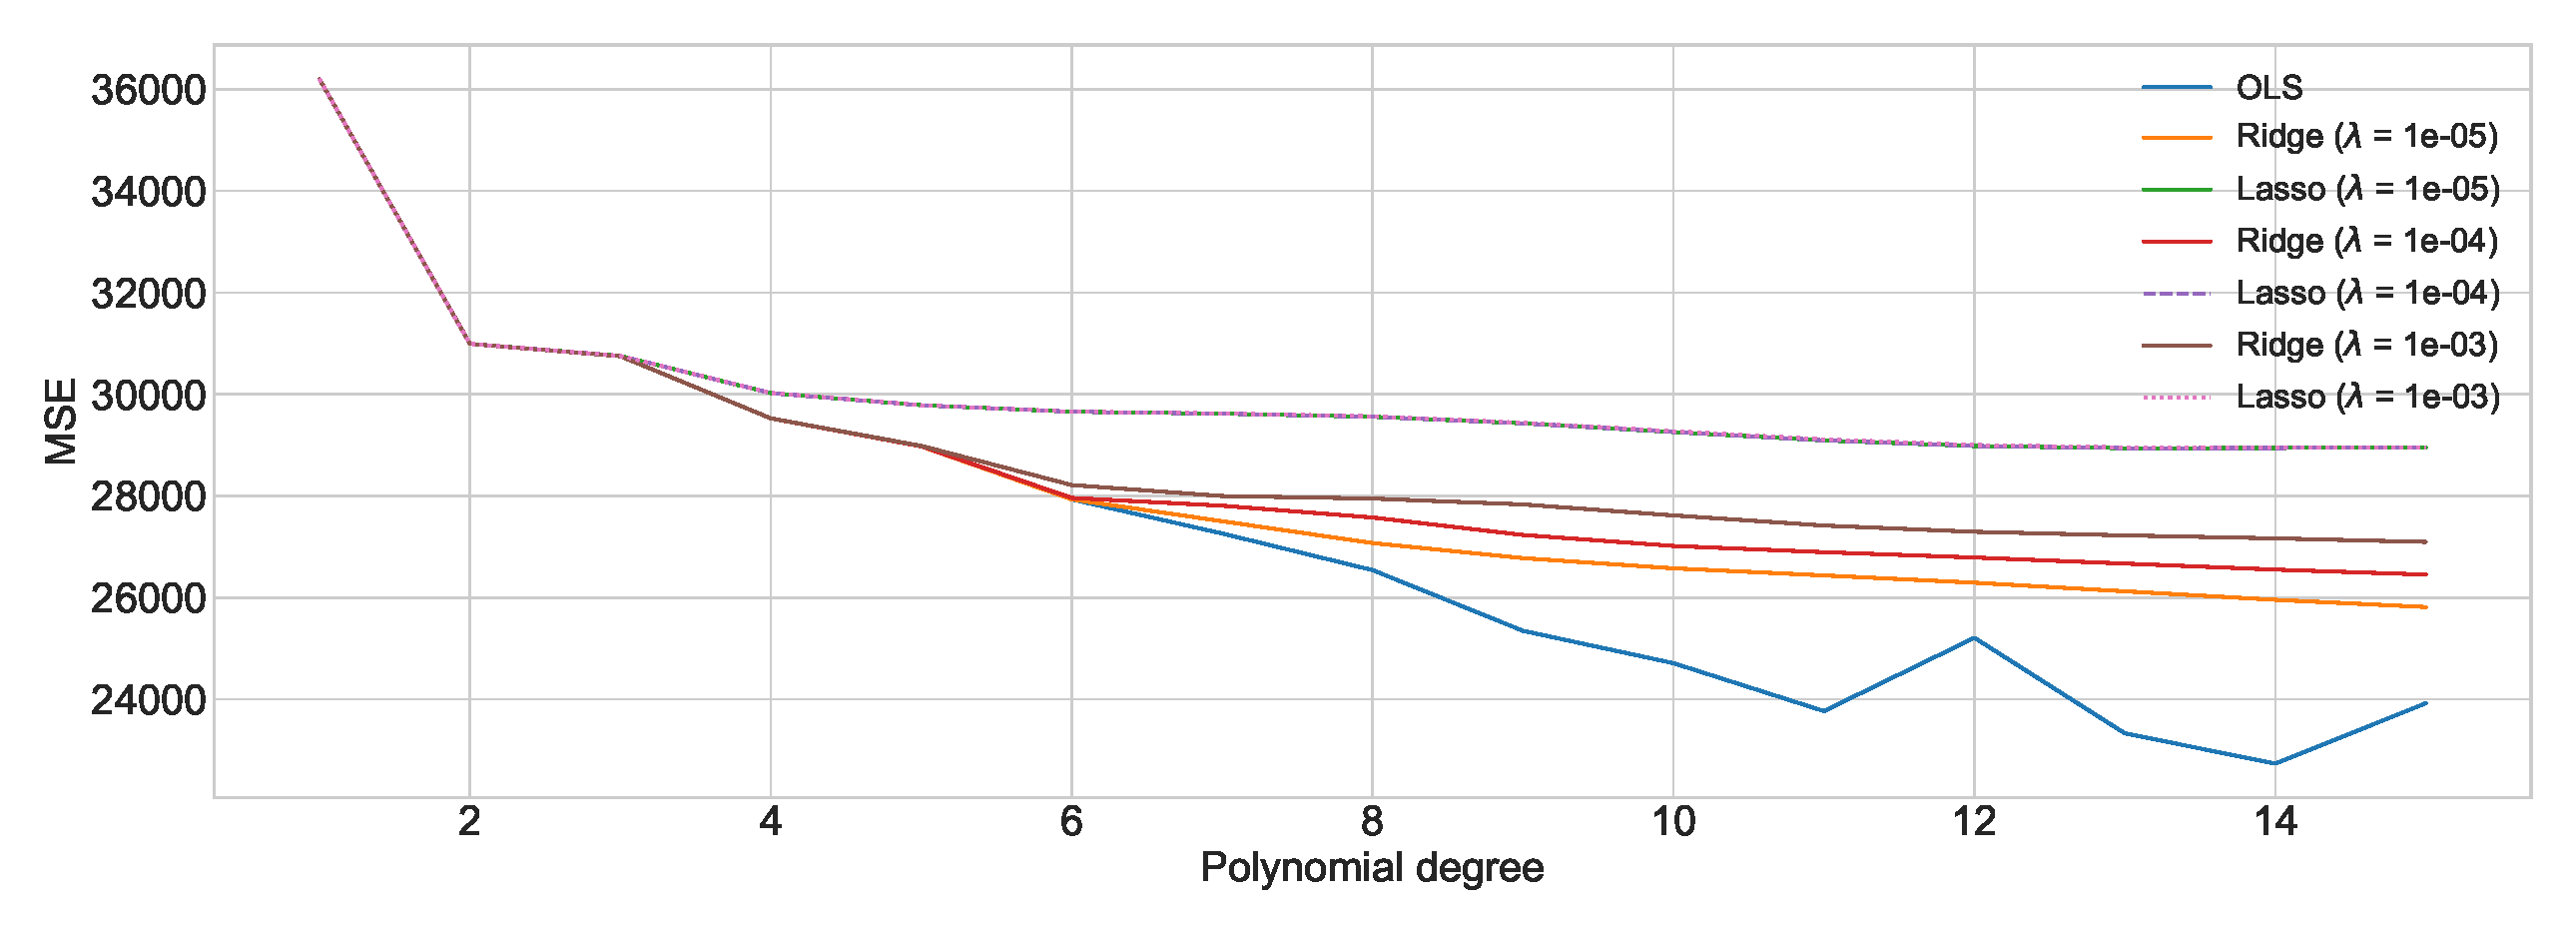
\includegraphics[width=1\linewidth]{images/part_g_real_data_mse_ols_ridge_lasso.pdf}
    \caption{The mean squared error for OLS, Ridge and Lasso regression performed on the real terrain data}
    \label{fig:part_g_real_data_mse_ols_ridge_lasso}
\end{figure}

As a closing note, we present the real topographic data used in \autoref{fig:part_g_real_data}, and an image plot of the fitted version in \autoref{fig:part_g_fit_data_deg100_plot}, using a polynomial of degree 100 trained with OLS regression.  

\begin{figure}
    \centering
    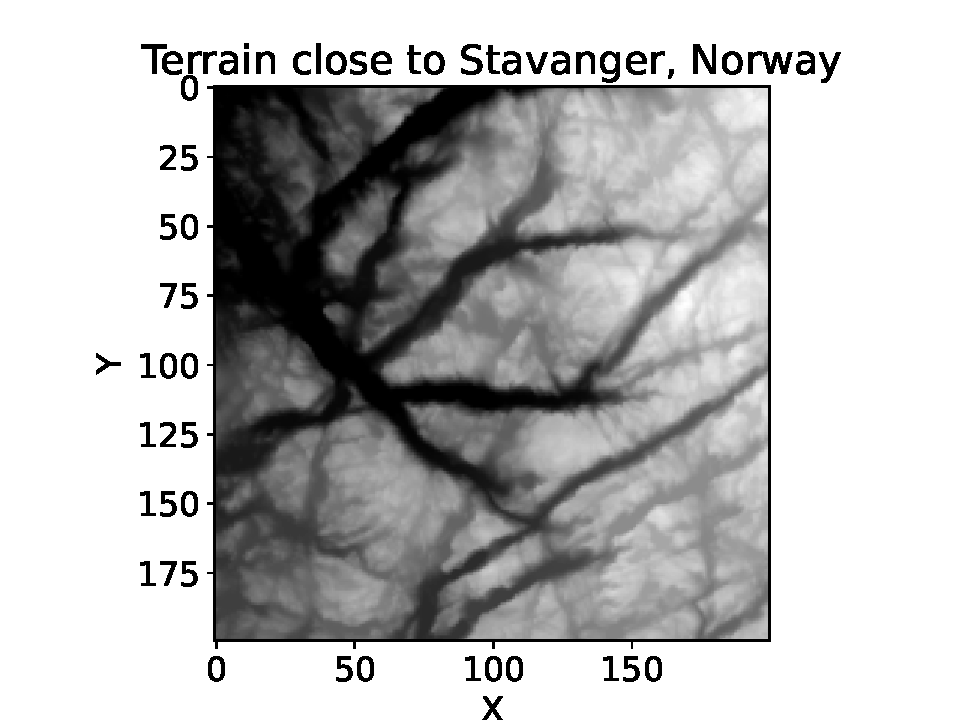
\includegraphics[width=0.8\linewidth]{images/part_g_real_data.pdf}
    \caption{Real topographic data of terrain close to Stavanger, Norway.}
    \label{fig:part_g_real_data}
\end{figure}


\begin{figure}
    \centering
    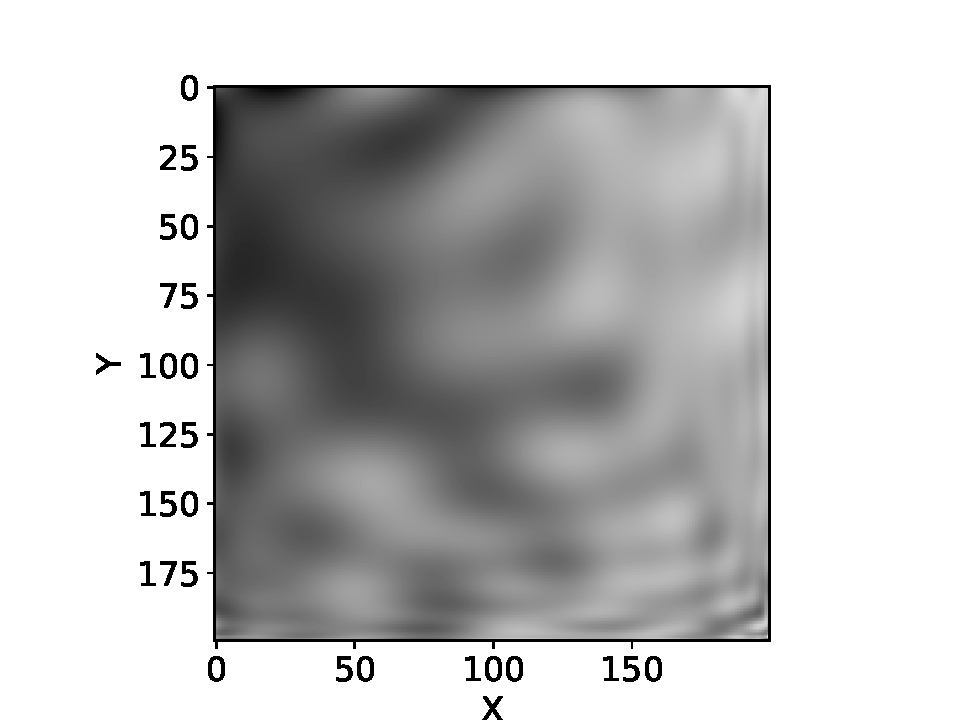
\includegraphics[width=0.8\linewidth]{images/part_g_fit_data_deg100_plot.pdf}
    \caption{Polynomial of trained OLS regression model with polynomial degree 100.}
    \label{fig:part_g_fit_data_deg100_plot}
\end{figure}

\newpage
\section{Discussion} \label{sec:discussion}

When fitting both the Franke function and the real-world data, we saw a clear trend that ordinary least squares was performing very well when compared to Ridge and Lasso regression. The closest fits to that of OLS was often Ridge and Lasso regression with small values of $\lambda$, naturally because Ridge and Lasso regression approaches OLS when $\lambda$ goes towards zero. Additionally, we did see a steady trend of error decreasing as the complexity of the model increased, and we did not seem to run into the problem of overfitting, as the models still had the best predictions on the test data for higher order polynomials. This is perhaps one of the factors contributing to OLS performing the best, as regularization such as Ridge and Lasso are often used to penalize complexity and avoid overfitting, but if our model is not overfit, then OLS can perform very well on its own. An example of this penalization can be seen clearly when comparing the $\boldsymbol{\beta}$ values in \autoref{fig:part_a_beta_vals} and \autoref{fig:part_b_beta_vals}, where Ridge regression constricts the spread of the values for $\beta$, relative to their values for low complexity. Meanwhile, the $\boldsymbol{\beta}$ values for the OLS regression can be seen to increase with increasing degrees of complexity of the model. The poorest performance came from Ridge and Lasso regression with the largest values for $\lambda$.

In regards to the bias-variance tradeoff, we can see a trend of the variance increasing for the more complex models in \autoref{fig:part_e_bias_var_21x21}. Although the bias makes up the majority of the MSE, we see that the variance becomes significant above polynomial degree 8. This plot shows that the best bias-variance tradeoff is found for polynomial degrees 3 to 8. The problem of high variance is almost completely alleviated in \autoref{fig:part_e_bias_var_101x101}, because with a data set of $101\times101$ points, bootstrapped 10 times, the statistics are stable enough that training yields close to the same model every bootstrap iteration for these levels of complexity.

When comparing the bootstrap method to cross-validation in \autoref{fig:part_f_MSE_10bootstraps_10fold_crossval}, we can see that the bootstrap method has a slightly faster drop in error, but starts to flatten out, earlier, and even has a slight increase in error for higher order polynomials. Cross-validation seems to decrease steadily as complexity of the model increases. Generally, cross-validation is less biased than bootstrap as an estimator for the error, but has higher variance \cite{CV-Boot}. This poses a possible explanation for cross-validation providing a lower error estimate than bootstrapping, if our data set is large enough to account for variance. 

When applying our model to the real terrain data, the general trend is that higher order polynomials fit the data best, and OLS outperformed the other models, followed by Ridge for increasing values of $\lambda$. Lasso regression gave the highest MSE, which was close to equal for the different values of $\lambda$. The absolute best fit was found for OLS with a polynomial of degree 14, although the slight increase for degree 15 may possibly be attributed to chance. By comparing the image of the real data in \autoref{fig:part_g_real_data} against the fitted function of polynomial degree 100 in \autoref{fig:part_g_fit_data_deg100_plot}, we observe general similarities in the values of the two images, but the polynomial function is unable to obtain the finer details observed in the real data. Considering that this fit was performed using a polynomial of degree 100, this suggests that regression using a polynomial function is not suited for capturing the finer details of such terrain data.

\section{Conclusion} \label{sec:conclusion}
We have explored different linear regression models, which were applied to data from the Franke function and real terrain data. We found that ordinary least squares provided the best fit to these data sets. This indicates that we did not encounter the problem of overfitting, even for the highest order polynomials, as the regularization techniques Ridge and Lasso regression consistently provided higher MSE than OLS.  

We also found that cross-validation provided a lower error than bootstrapping, except for the models with the lowest complexity. 

Future work could include further investigations into higher order polynomials, to see if overfitting eventually becomes a problem, where Ridge and Lasso regression might overtake OLS.
One could also investigate further which complexity is needed to more accurately represent the real data, and if a polynomial is a sufficiently complex model at all. 

\printbibliography

\end{document}
